
%---------------------导言区---------------------------%
\documentclass[12pt,a4paper,UTF8]{ctexart}
	%10pt:正文字体为12pt,缺省为10pt;各层级字体大小会根据正文字体自动调整
	%a4paper:纸张大小a4;
	%UTF8:中文要求
\usepackage{geometry}%用于设置上下左右页边距
	\geometry{left=2.5cm,right=2.5cm,top=3.2cm,bottom=2.8cm}
\usepackage{xeCJK,amsmath,paralist,enumerate,booktabs,multirow,graphicx,subfig,setspace,listings,lastpage,hyperref,setspace}
	%xeCJK:中文字体(如楷体,作者和机构需要用到)的设置
	%amsmath:数学公式
	%paralist,enumerate:自定义项目符号
	%booktabs:三线图,论文常用的表格风格
	%multirow:复杂表格
	%graphicx,float: 插入图片
	%subfig:并排排版图片、竖向排版图片
	%setspace:设置行间距等功能
	\setlength{\parindent}{2em}%正文首行缩进两个汉字
	%listings:用于排版各种代码;比如matlab的代码
	\lstset{language=Matlab}%matlab代码
	%lastpage:获取总页数;
	%hyperref:超链接,和lastpage搭配.
\usepackage{fancyhdr}
	%fancyhdr:一个很强大的宏包,用于自定义设计页面风格并命名以供调用。
	\pagestyle{fancy}
	\rhead{实验C3.1 原子发射光谱的观测}
	\lhead{基础物理实验\uppercase\expandafter{\romannumeral2}会议摘要}
	\cfoot{Page \thepage/\pageref{LastPage}}  %当前页\总页数
		%分别是右页眉、左页眉、中页脚、右页脚
	\renewcommand{\headrulewidth}{0.4pt}
	\renewcommand{\theenumi}{(\arabic{enumi})}
	\setlength\headheight{15pt}

\begin{document}

%%begin-------------------标题与信息-----------------------%%

%%标题
\begin{center}
\LARGE\textbf{实验C3.1 原子发射光谱的观测}
\end{center}

%%信息
\begin{doublespacing}
	%doublespacing:手动两倍行距
	\centering
	\begin{tabular}{lr}
	& \\
	{\CJKfontspec{方正楷体简体} 实验人姓名、学号:莫润冰~20980131} & {\CJKfontspec{方正楷体简体}合作者姓名、学号:黄健祥~20980118}\\
	\end{tabular}
\end{doublespacing}

%%end-------------------标题与信息-----------------------%%
\doublespacing
	\vspace{4em}
	%vspace:调整垂直空白,可以自己调整;缩小abstract和center(以及maketitle)的间距
	%\noindent %备用:摘要无缩进
	{\bf 摘{} 要:}
	{\zihao{-4} 根据玻尔的理论,原子由一个能级跃迁至另一能级时,会吸收或辐射一定能量的光子,而光子的能量等于两个能级之间的能级差。
	这一理论成功解释了氢原子光谱不连续的特点,计算出氢原子的轨道半径并成为物理发展史上一个重要的里程碑,对于以后建立量子力学理论起了巨大的推动作用。
	光栅光谱仪是测量物质光谱的仪器,除了发射光谱的测量,光栅光谱仪在物质组分与结构分析方面有着广泛的应用。
	
	在本实验中,我们用光栅光谱仪测量汞灯、钠灯、溴钨灯、氢氘灯和各色LED灯(红、黄、绿、蓝、白)的发射光谱,发现其中汞灯,钠灯和氢氘灯光谱为分立谱,而溴钨灯和五种颜色 LED 灯光谱为连续谱。
	对其中的分立谱,我们将其峰值波长与标准值标定;对于连续谱,我们使用高斯函数拟合计算波包中心峰值波长后标定。

	}
	\par%空的新行的高度。
	\textbf{关键词}:光栅光谱仪,发射光谱
	\vspace{3em}

\newpage

	\renewcommand{\abstractname} {} %不显示摘要名字
	\begin{center}%
	    {\LARGE\bfseries Experiment C3.1: Observation of atomic emission spectra\footnotemark[1]  \par}%
	    \vskip 1.4em%
	    {\large
	    \lineskip .75em%
	    \begin{tabular}[t]{c}%
	        \large Runbing Mo$^{1}$
	    \end{tabular}\footnotemark[2] \par
	    }%
	    \vskip 0.4em%
	    {\normalsize School of Medicine, Sun Yat-sen University, Guangzhou  { \rm 510275}, China}
	\end{center}
	\begin{abstract}
		\vspace{-2em}  %缩小abstract和center(以及maketitle)的间距
	    	{\bf Abstract:}
			{According to Bohr's theory, when an atom jumps from one energy level to another, it absorbs or radiates photons of energy which equals to the difference between the two levels.
			This theory successfully explained the characteristic of discontinuous spectrum of hydrogen atom, thus having calculated the orbital radius of hydrogen atom.
			Since then it became an important milestone in the history of physics, which played a great role in promoting the establishment of quantum mechanics theory in the future.
			Grating spectrometer is an instrument to measure the spectrum of matter. In addition to the measurement of emission spectrum, grating spectrometer has a wide range of applications in the analysis of material composition and structure.

			In this experiment, we measured the emission spectra of mercury lamp, sodium lamp, bromine tungsten lamp, hydrogen deuterium lamp and various LED lights (red, yellow, green, blue and white) with a grating spectrometer.
			We found that the spectra of mercury lamp, sodium lamp and hydrogen deuterium lamp are discrete, while the spectra of bromine tungsten lamp and LED lights were continuous.
			For discrete spectrum, we calibrated its peak wavelength with standard value. For continuous spectrum, we use Gaussian function fitting to calculate the peak wavelength before calibration}
			\par%空的新行的高度。
		\textbf{Key words}: Grating spectrometer, Emission spectrum
	\end{abstract}
\footnotetext[1]{{Supported and taught by Han Shen, School of Physics, Sun Yat-sen University}}
\footnotetext[2]{{Corresponding author. E-mail:\url{morb@mail2.sysu.edu.cn}}}


\newpage
\subsection*{【实验参数】}
\begin{table}[htbp]
	\caption{实验参数}
	\centering
    \begin{tabular}{cccc}
	\toprule
    光源类型 &起始波长(nm)&终止波长(nm)&扫描间隔(nm)\\
	\midrule
	汞灯&300&700&0.1\\
	钠灯&586&590.5&0.01\\
    氢氘灯&300&700&0.1\\
	溴钨灯&300&700&0.2\\
	红光&550&690&0.1\\
	黄光&550&650&0.1\\
	绿光&460&605&0.1\\
	蓝光&400&530&0.1\\
	白光&390&630&0.1\\
	\bottomrule
	\end{tabular}%
	\label{tab:data}%
\end{table}%


\subsection*{【数据处理】}
\subsubsection*{1.汞灯发射光谱}
由origin软件作出汞灯的发射光谱图1

\begin{figure}[htbp]
	\centering
	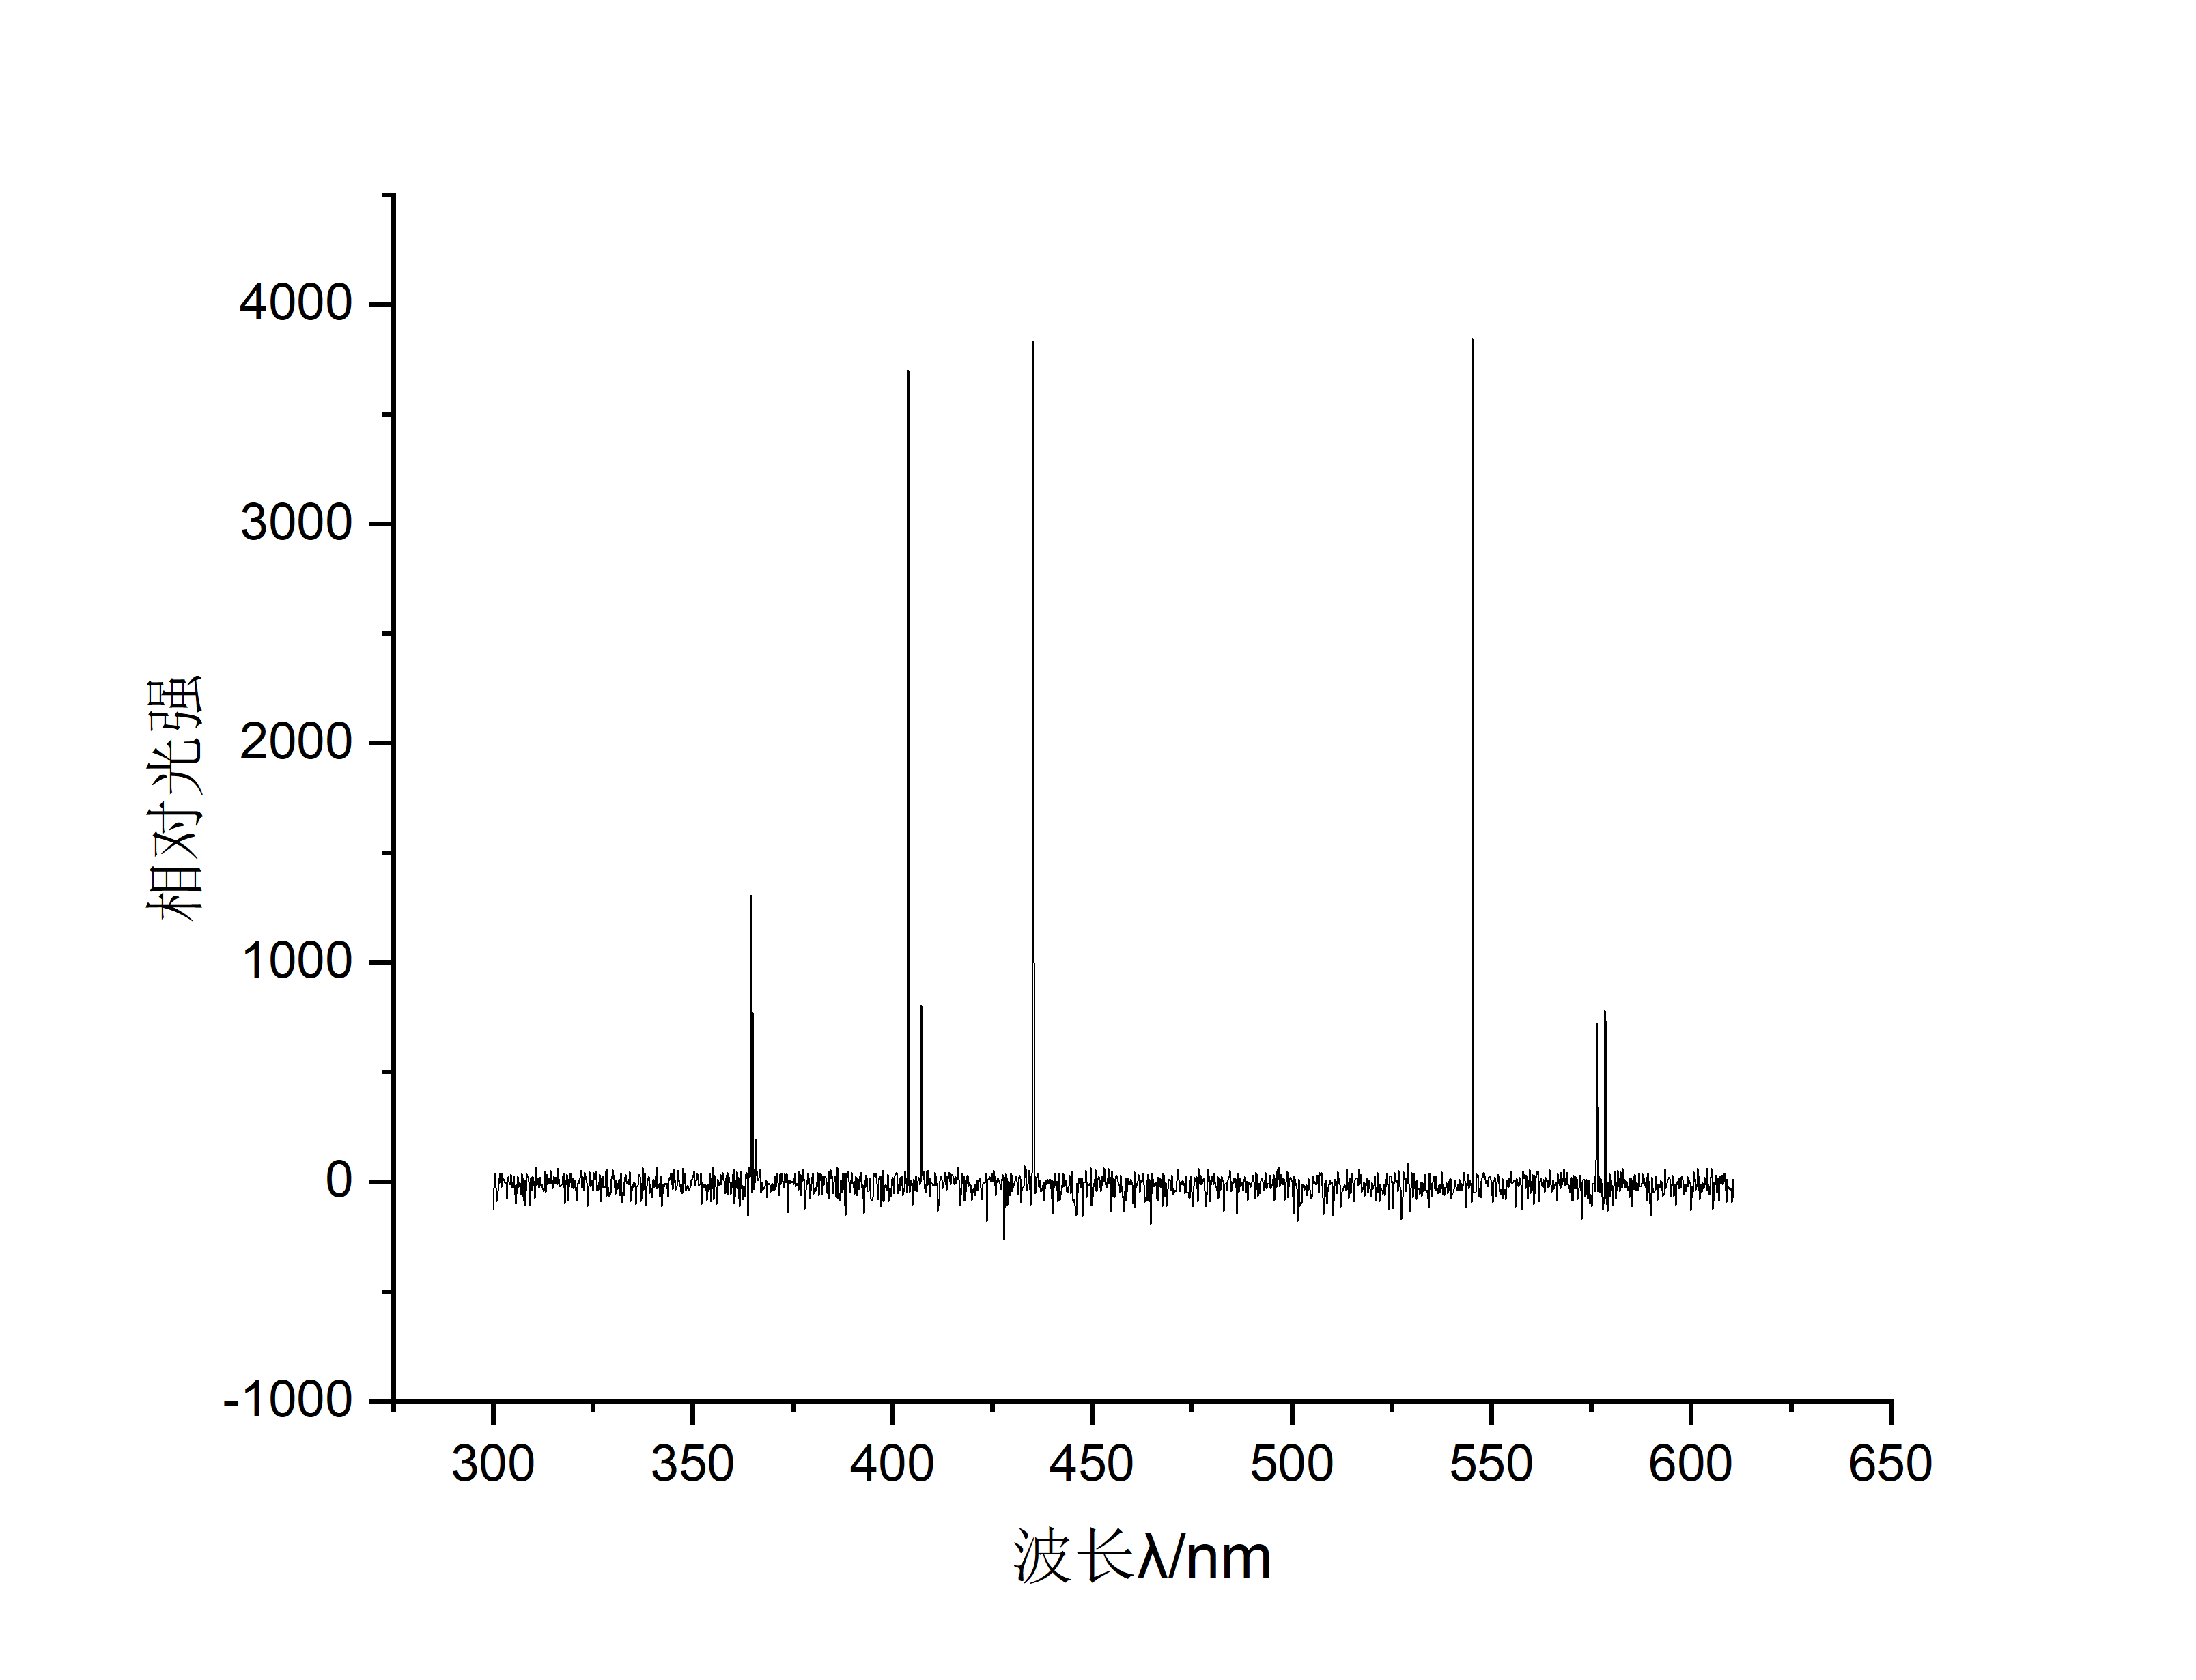
\includegraphics[width=0.7\textwidth]{img//Hg.png}
	\caption{汞灯发射光谱图}
	\label{fig:1}
\end{figure}


用Origin软件的快速寻峰功能可得汞灯光谱峰值,查阅资料得标准峰值数据,具体数据见图2、表3。

\begin{figure}[htbp]
	\centering
	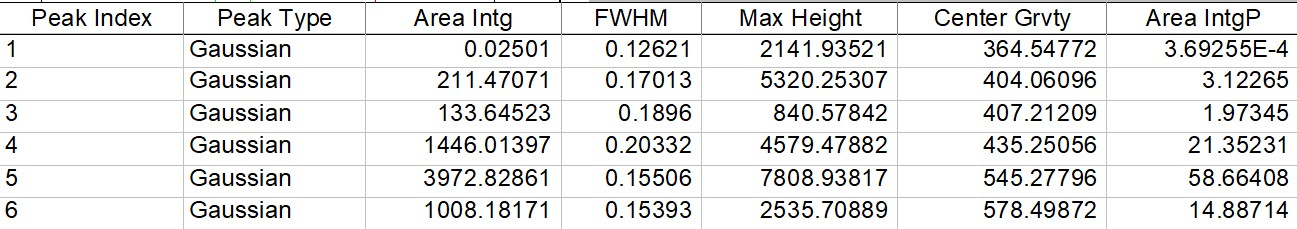
\includegraphics[width=\textwidth]{img//Hgpeak.jpg}
	\caption{汞灯发射光谱峰值信息}
	\label{fig:2}
\end{figure}


\begin{table}[htbp]
	\caption{1.汞灯光谱数据}
	\centering
    \begin{tabular}{cccccc}
	\toprule
    实验峰值波长$\lambda$(nm)&364.5&404.1&435.3&545.3&578.5\\
	\midrule
	标准峰值波长$\lambda_0$(nm)&365&404.0&435.2&546.6&576.5\\
	\bottomrule
	\end{tabular}%
	\label{tab:1}%
\end{table}%

将表2数据进行线性拟合得图3:

\begin{figure}[htbp]
	\centering
	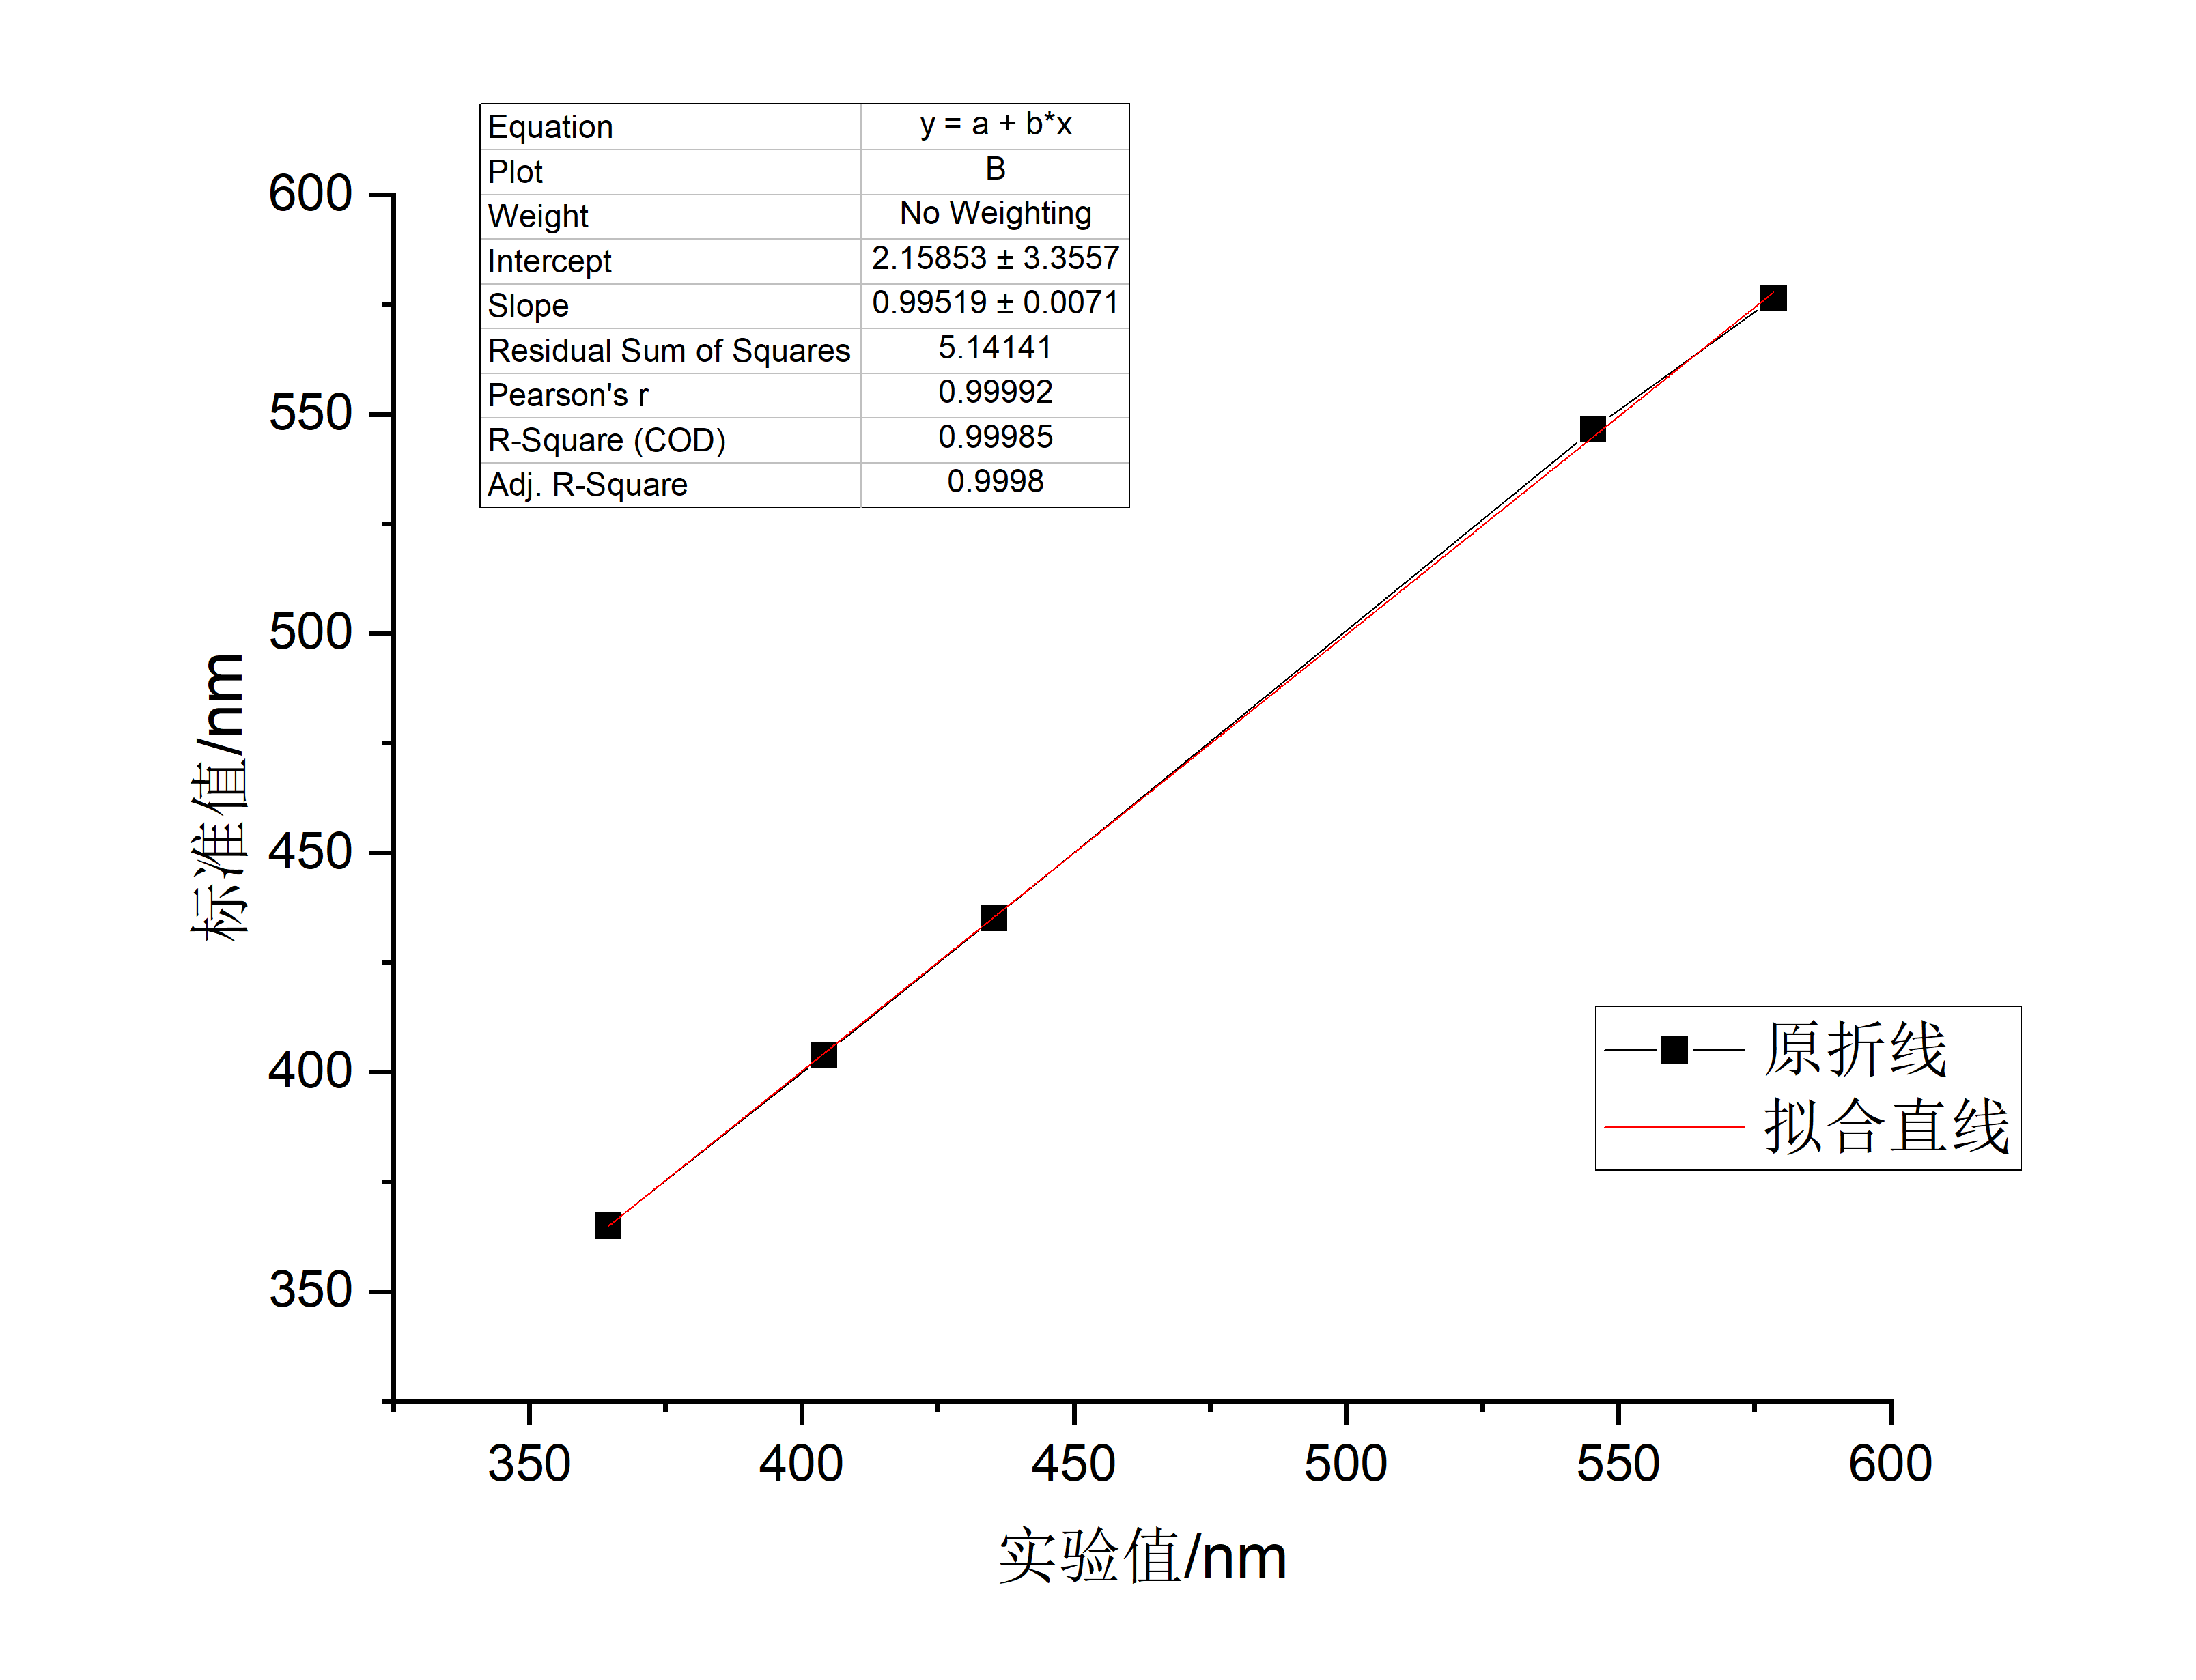
\includegraphics[width=0.8\textwidth]{img//LeanearReg.png}
	\caption{汞灯发射光谱峰值拟合}
	\label{fig:3}
\end{figure}



所得直线为:
\begin{equation*}
	y=0.99519x+2.15853
\end{equation*}

相关系数为0.99992,P<0.0001,线性关系良好。

\subsubsection*{2.钠灯发射光谱}
\begin{figure}[htbp]
	\centering
	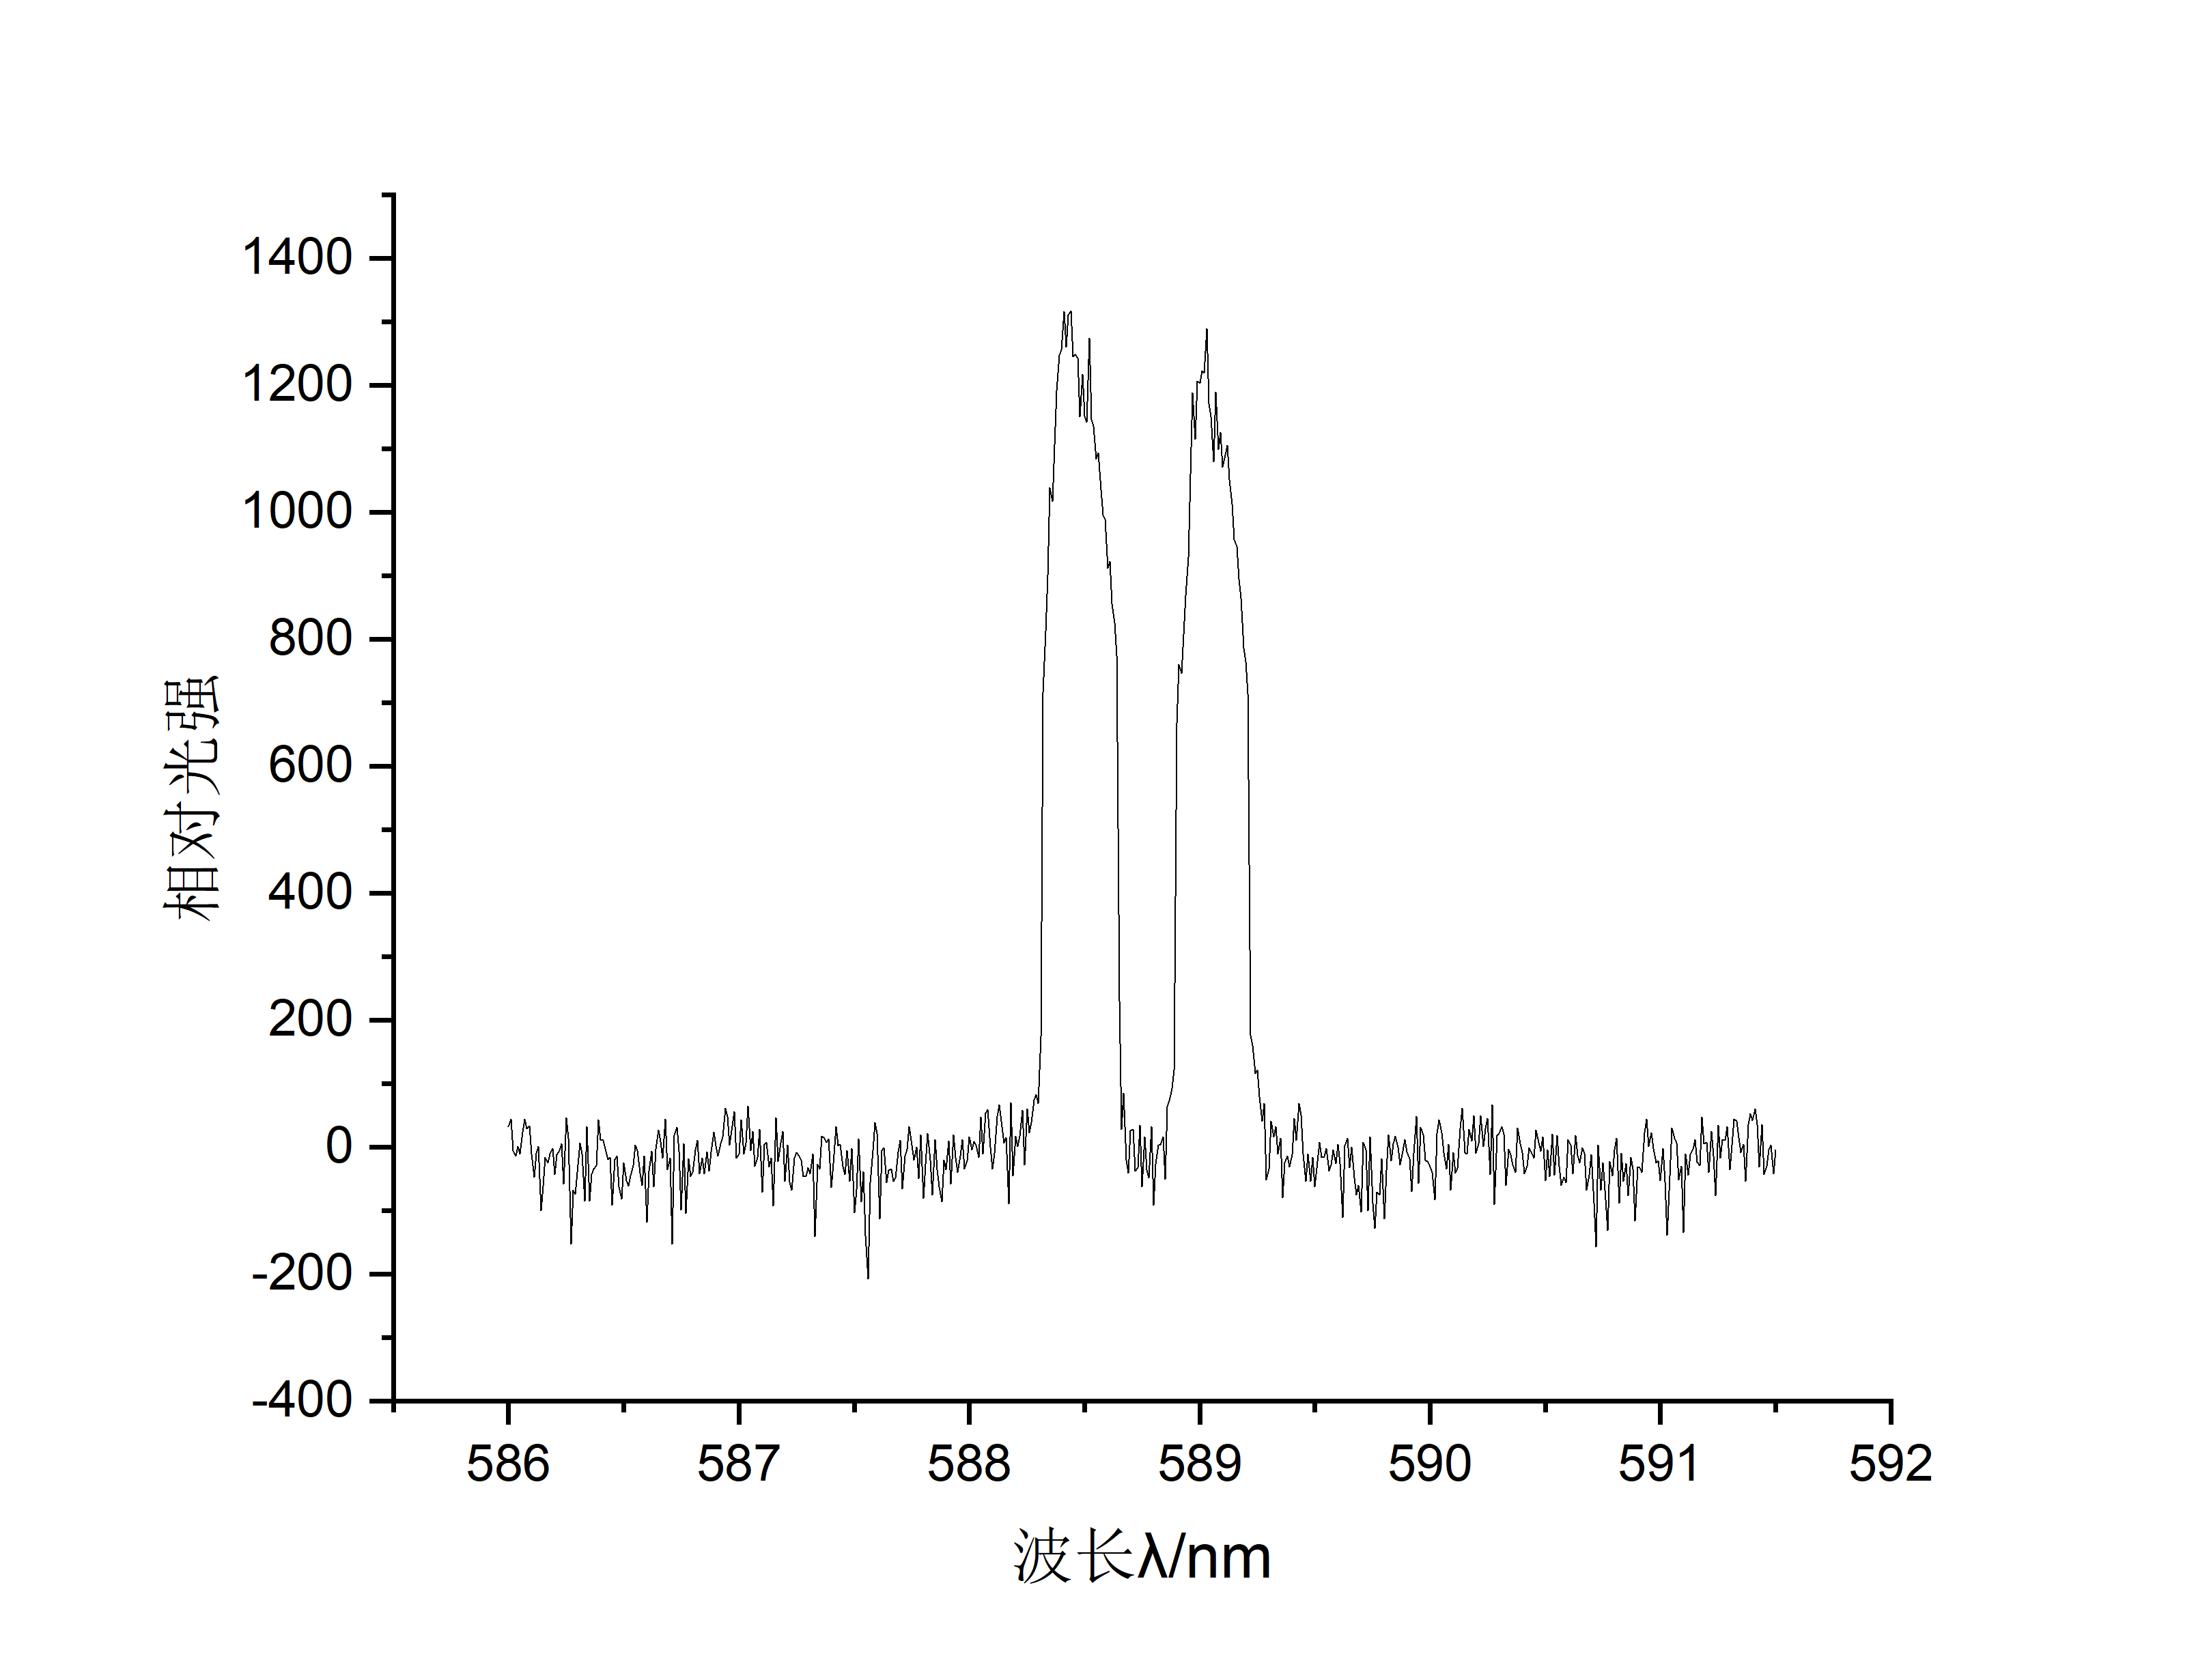
\includegraphics[width=0.7\textwidth]{img//Na.png}
	\caption{钠灯发射光谱}
	\label{fig:4}
\end{figure}

如图4,钠灯光谱峰值出现在$\lambda_1=588.40nm$,$\lambda_2=589.03nm$处,代入线性内插法拟合公式得Na双黄线实验谱线值为:
\begin{gather*}
	\lambda^{'}_1=0.99519\times\lambda_1+2.15853=587.73nm\\
    \lambda^{'}_2=0.99519\times\lambda_2+2.15853=588.36nm\\
\end{gather*}

由此得钠双黄线的波长差$\varDelta\lambda=0.63nm$

理论值$\varDelta\lambda_0=0.597nm$

相对误差:
\begin{equation*}
	\eta=(\frac{0.63}{0.597}-1)\times100\%=5.53\%
\end{equation*}

实验值与理论值有一定误差,但是相对误差较小,结果比较可信。

\subsubsection*{3.氢氘灯发射光谱}
\begin{figure}[htbp]
	\centering
	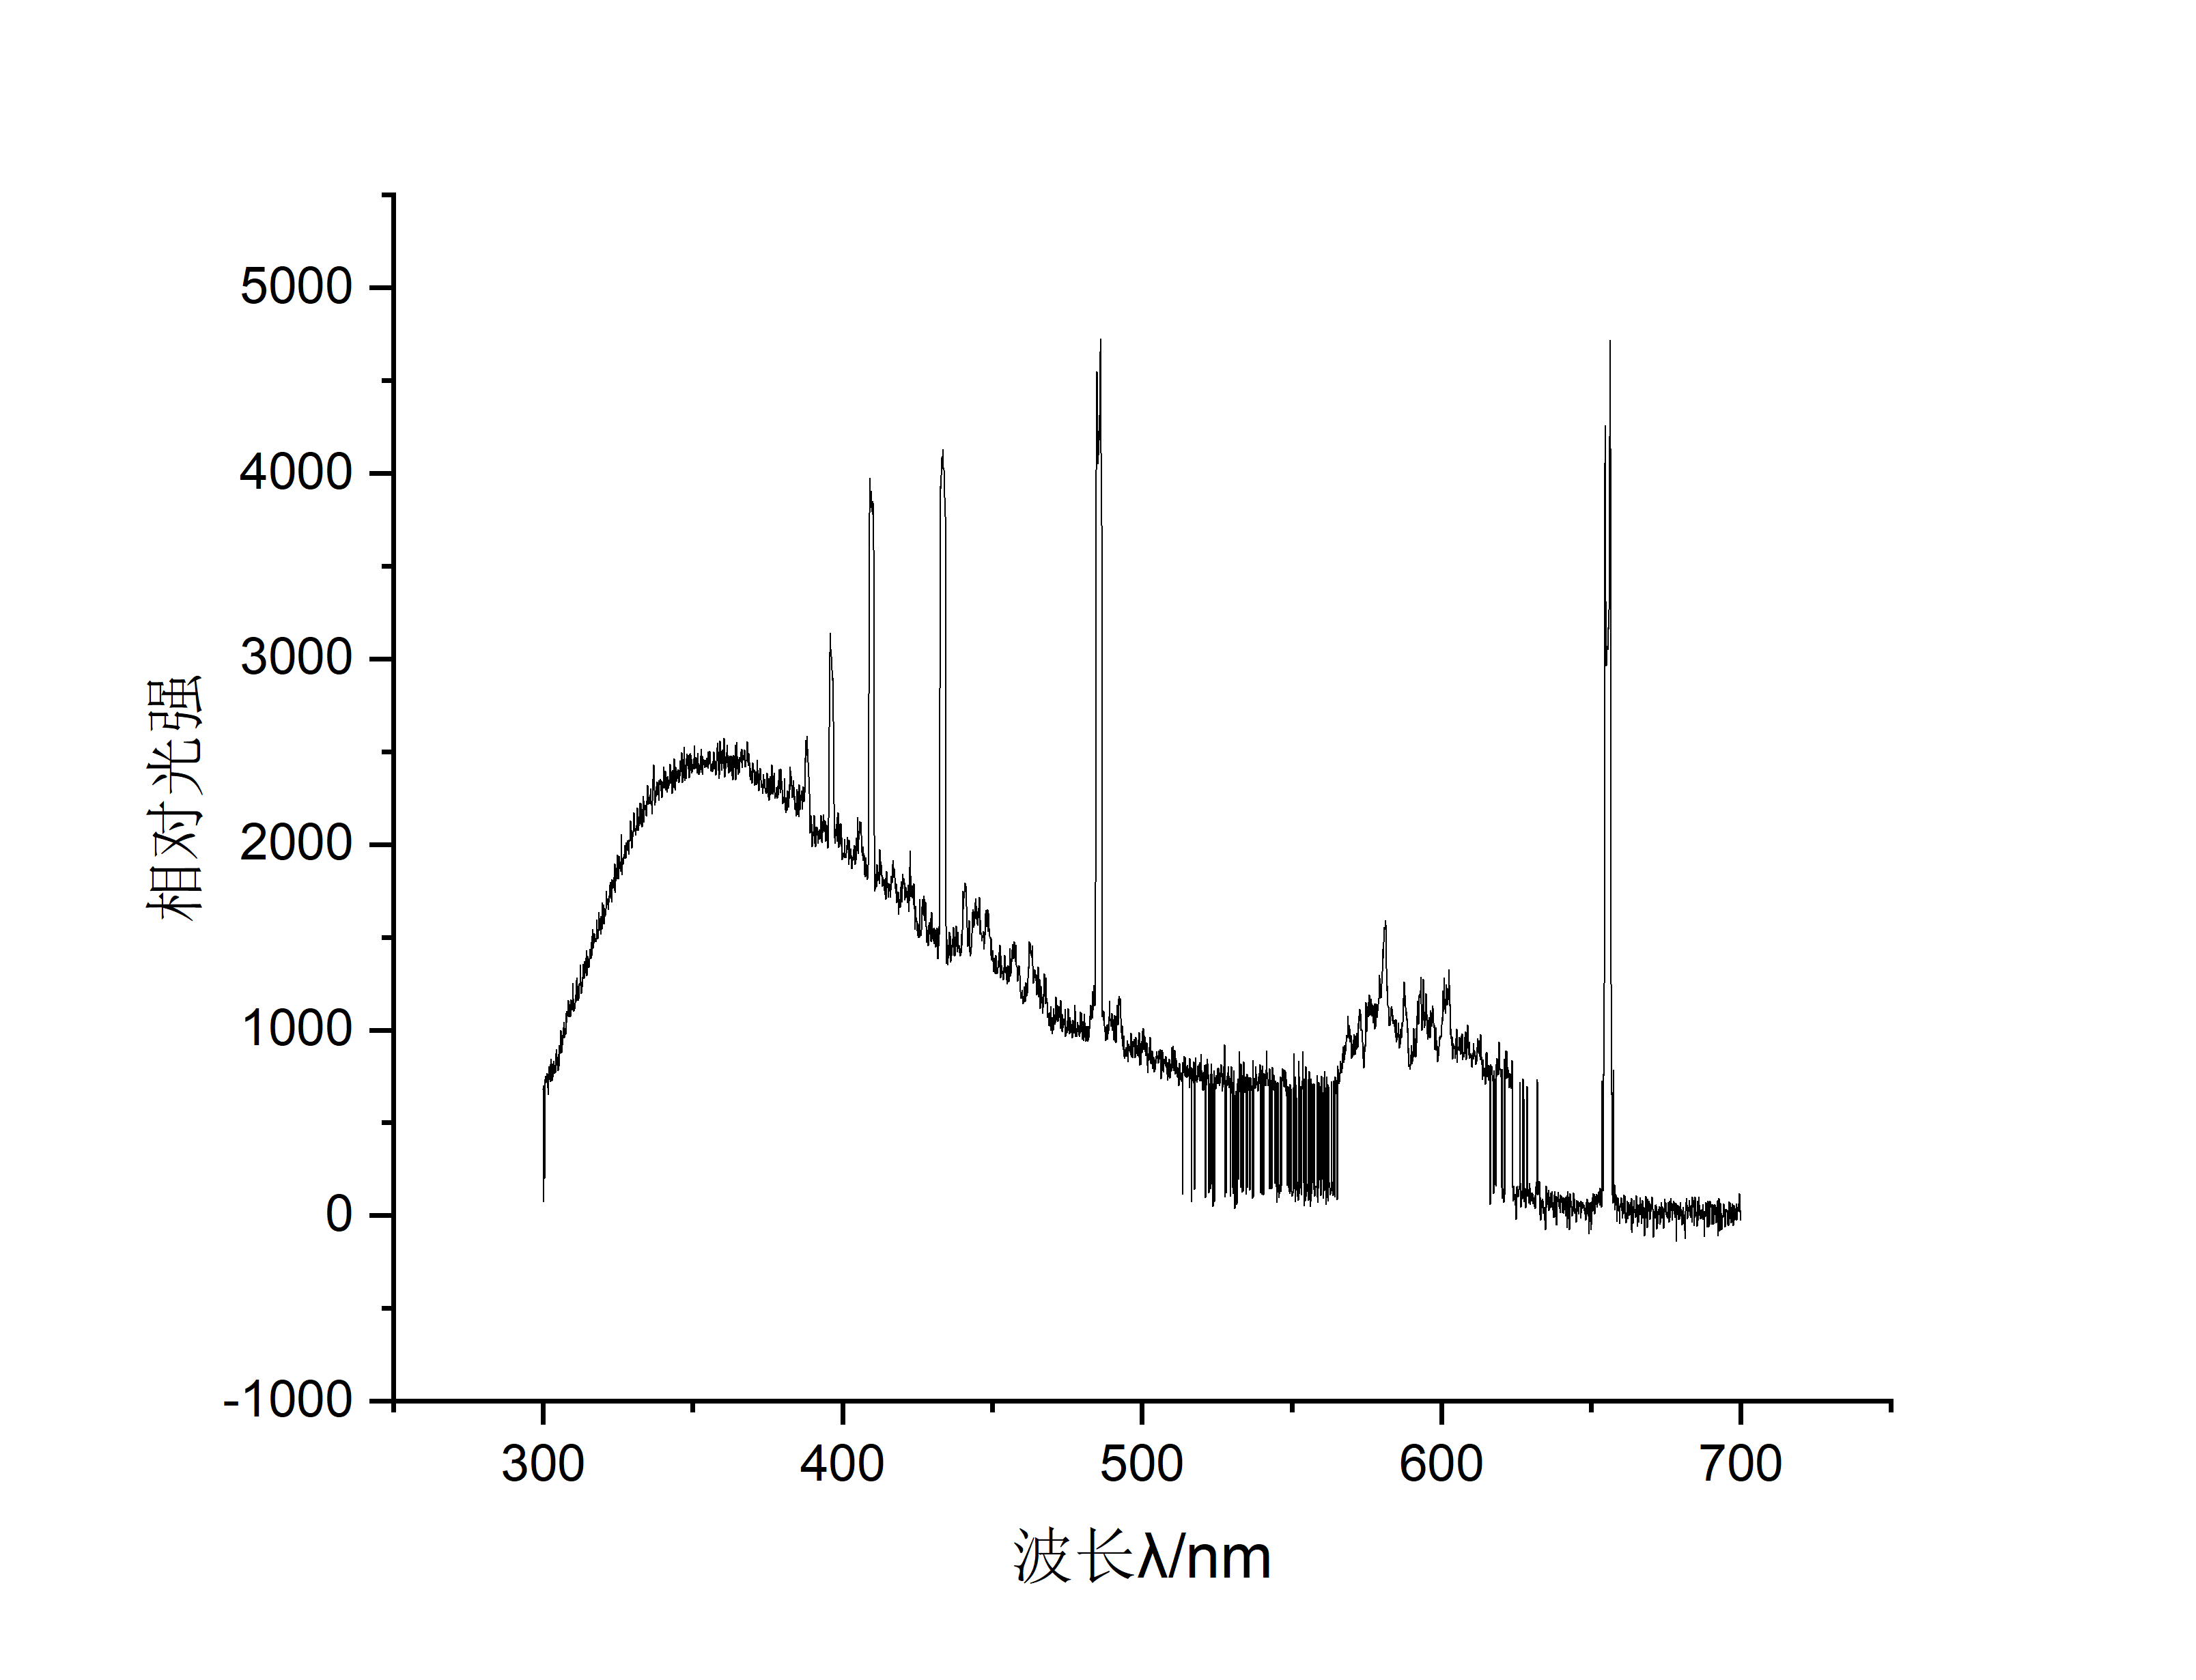
\includegraphics[width=0.7\textwidth]{img//HH.png}
	\caption{氢氘灯发射光谱}
	\label{fig:5}
\end{figure}


图5为实验扫描得氢氘灯发射光谱,由Origin软件快速标定功能可知峰值波长:
\begin{gather*}
	\lambda_1=395.92nm\\
	\lambda_2=409.34nm\\
	\lambda_3=433.21nm\\
	\lambda_4=486.23nm\\
	\lambda_5=656.29nm\\
\end{gather*}

代入线性内插法拟合公式得氢氘灯的实验谱线峰值为:
\begin{gather*}
	\lambda^{'}_1=0.99519\times\lambda_1+2.15853=396.17nm\\
	\lambda^{'}_2=0.99519\times\lambda_2+2.15853=409.53nm\\
	\lambda^{'}_3=0.99519\times\lambda_3+2.15853=433.28nm\\
	\lambda^{'}_4=0.99519\times\lambda_4+2.15853=486.05nm\\
	\lambda^{'}_5=0.99519\times\lambda_5+2.15853=655.29nm\\
\end{gather*}

查阅资料得,氢原子光谱的巴尔末系,其中对应的谱线波长如下:
\begin{gather*}
	\lambda_{10}=397.0nm\\
	\lambda_{20}=410.2nm\\
	\lambda_{30}=434.1nm\\
	\lambda_{40}=486.1nm\\
	\lambda_{50}=656.3nm\\
\end{gather*}

计算相对误差:
\begin{gather*}
	\sigma _1=\frac{|\lambda^{'}_1-\lambda_{10}|}{\lambda_{10}}\times100\%=0.21\%\\
	\sigma _2=\frac{|\lambda^{'}_2-\lambda_{20}|}{\lambda_{20}}\times100\%=0.16\%\\
	\sigma _3=\frac{|\lambda^{'}_3-\lambda_{30}|}{\lambda_{30}}\times100\%=0.19\%\\
	\sigma _4=\frac{|\lambda^{'}_4-\lambda_{40}|}{\lambda_{40}}\times100\%=0.01\%\\
	\sigma _5=\frac{|\lambda^{'}_5-\lambda_{50}|}{\lambda_{50}}\times100\%=0.15\%\\
\end{gather*}
实验误差较小,测量较准确。

\subsubsection*{4.溴钨灯发射光谱}
\begin{figure}[htbp]
	\centering
	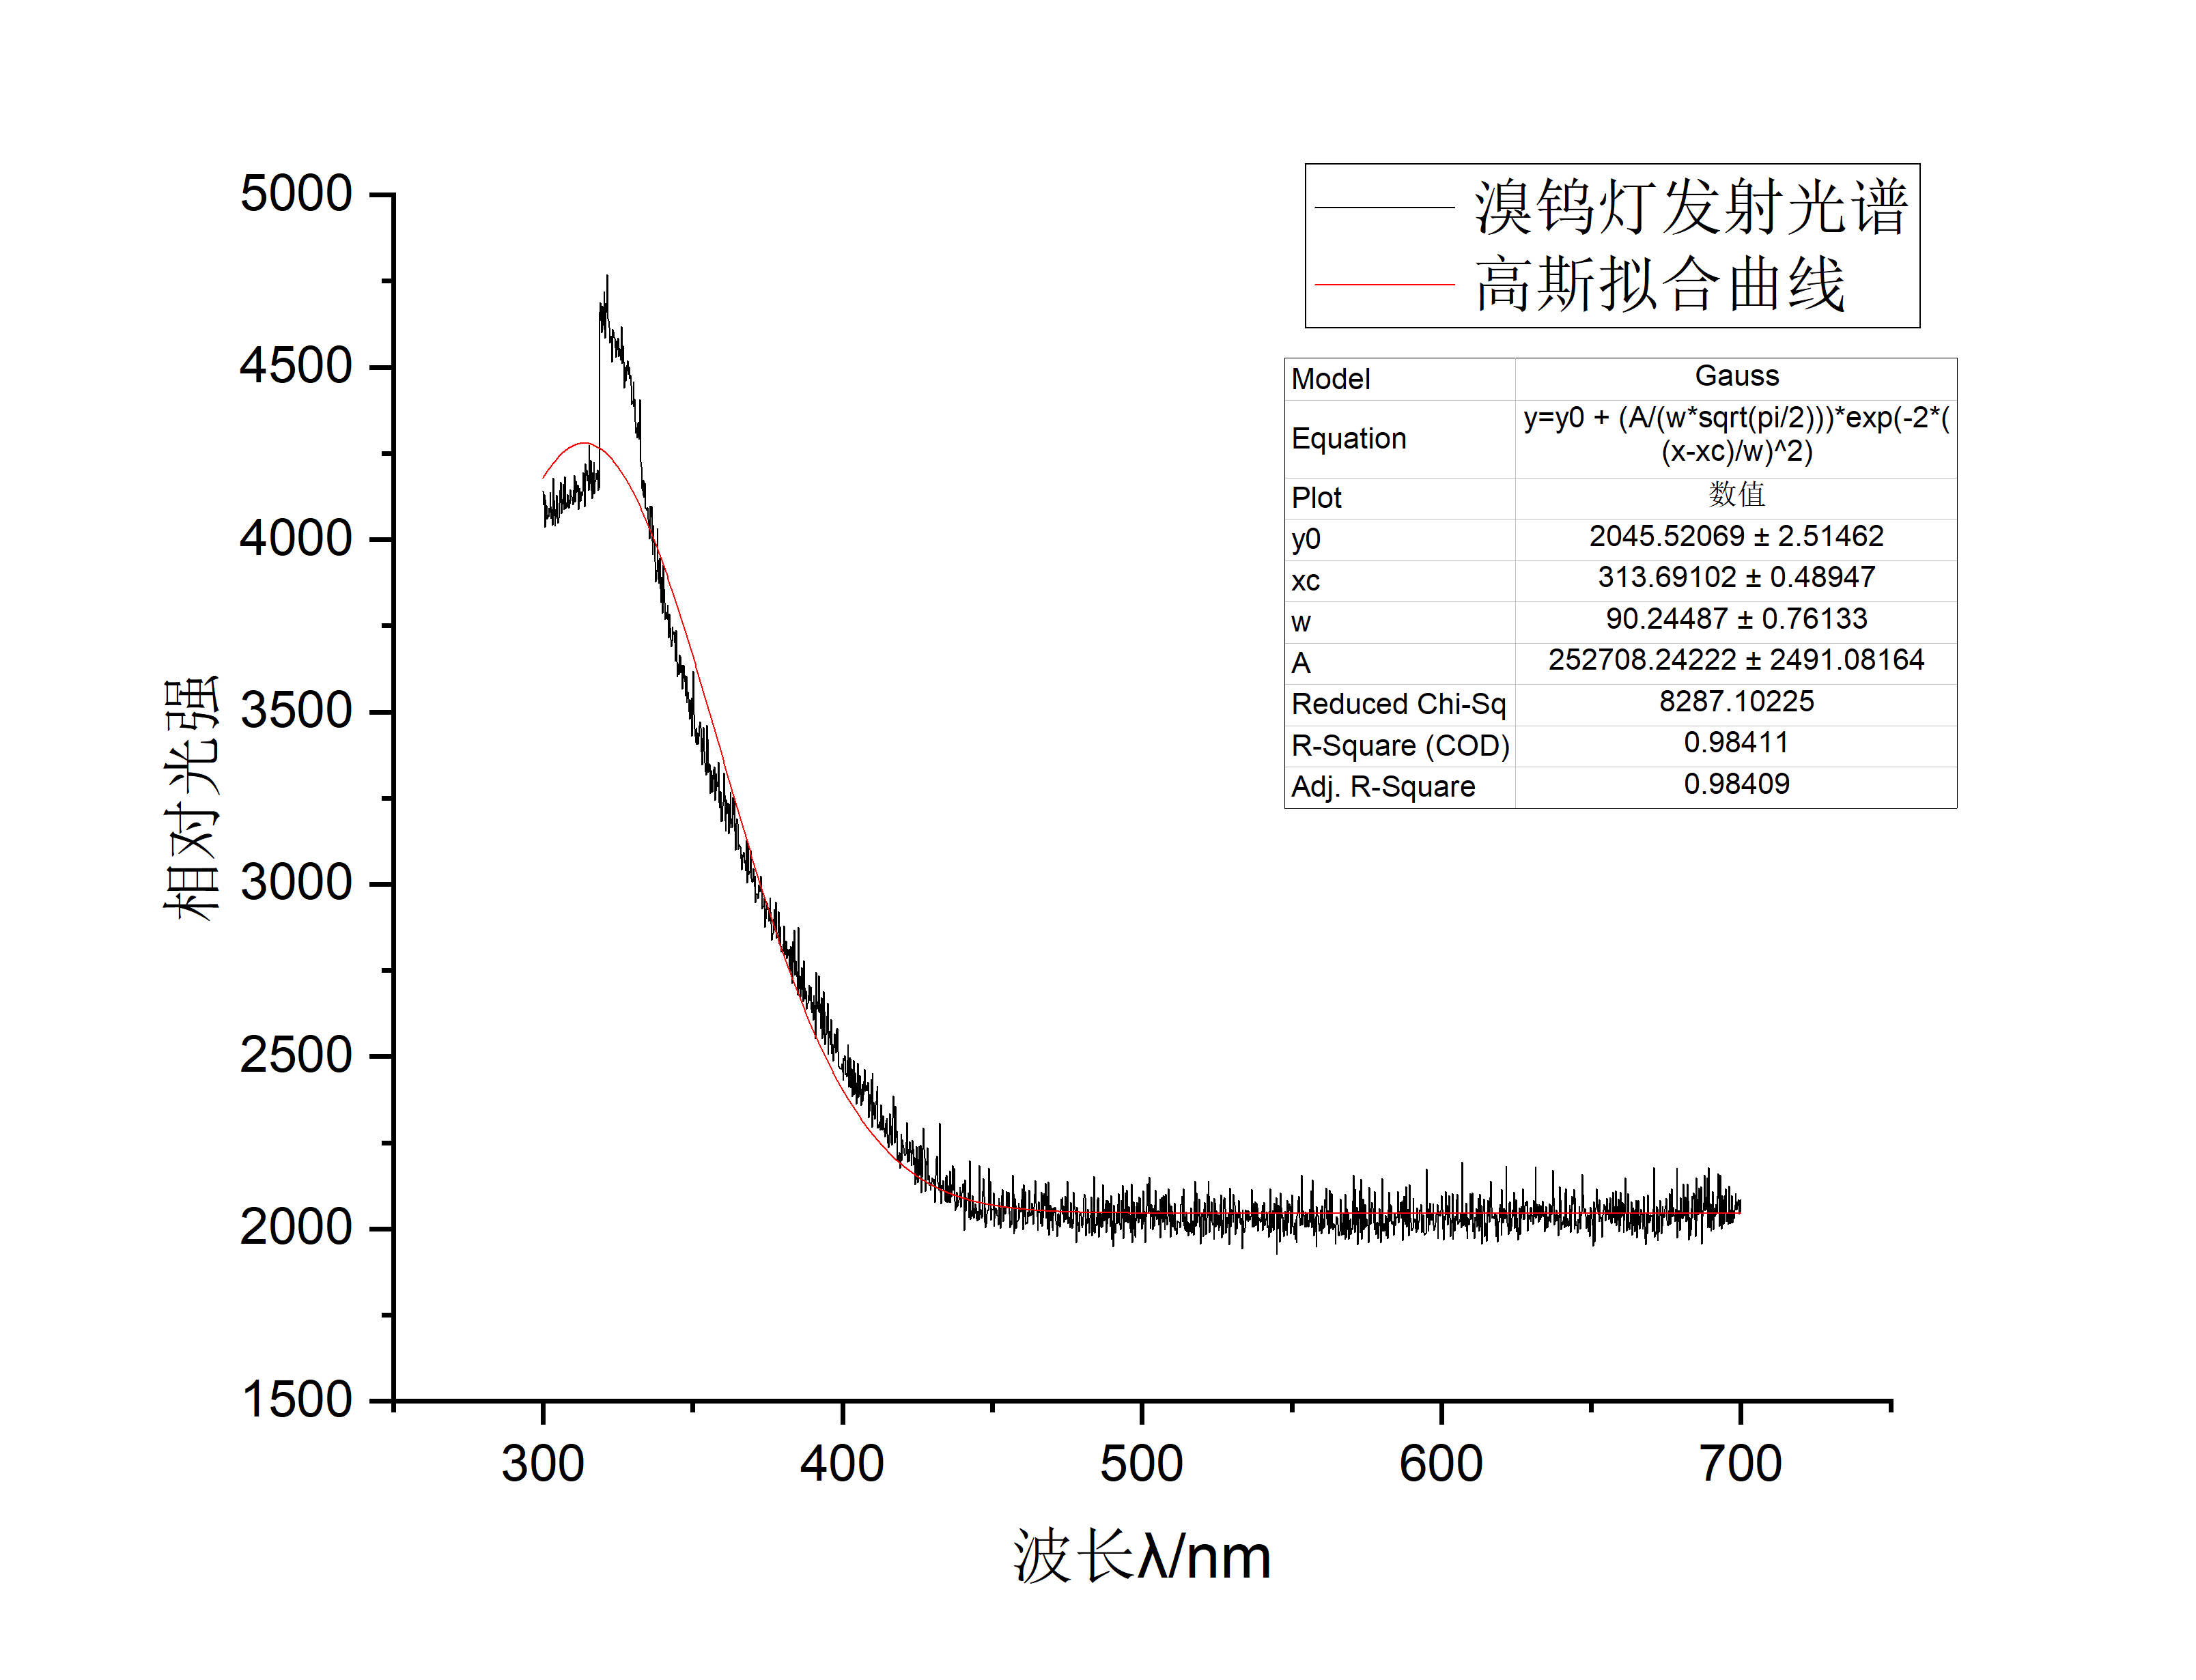
\includegraphics[width=0.7\textwidth]{img//BrWReg.png}
	\caption{溴钨灯发射光谱}
	\label{fig:7}
\end{figure}

由图7可知,溴钨灯发射光谱峰值并不尖锐,为连续光谱。通过高斯函数拟合发现,其峰值出现在313.69nm处。
通过线性插值法校正后波长为:
\begin{equation*}
	\lambda=0.99519\times313.69+2.15853=314.34nm
\end{equation*}

\subsubsection*{5.多种颜色LED发射光谱}
\begin{figure}[htbp]
	\centering
	\subfloat[红光]{\label{fig:8.1}
	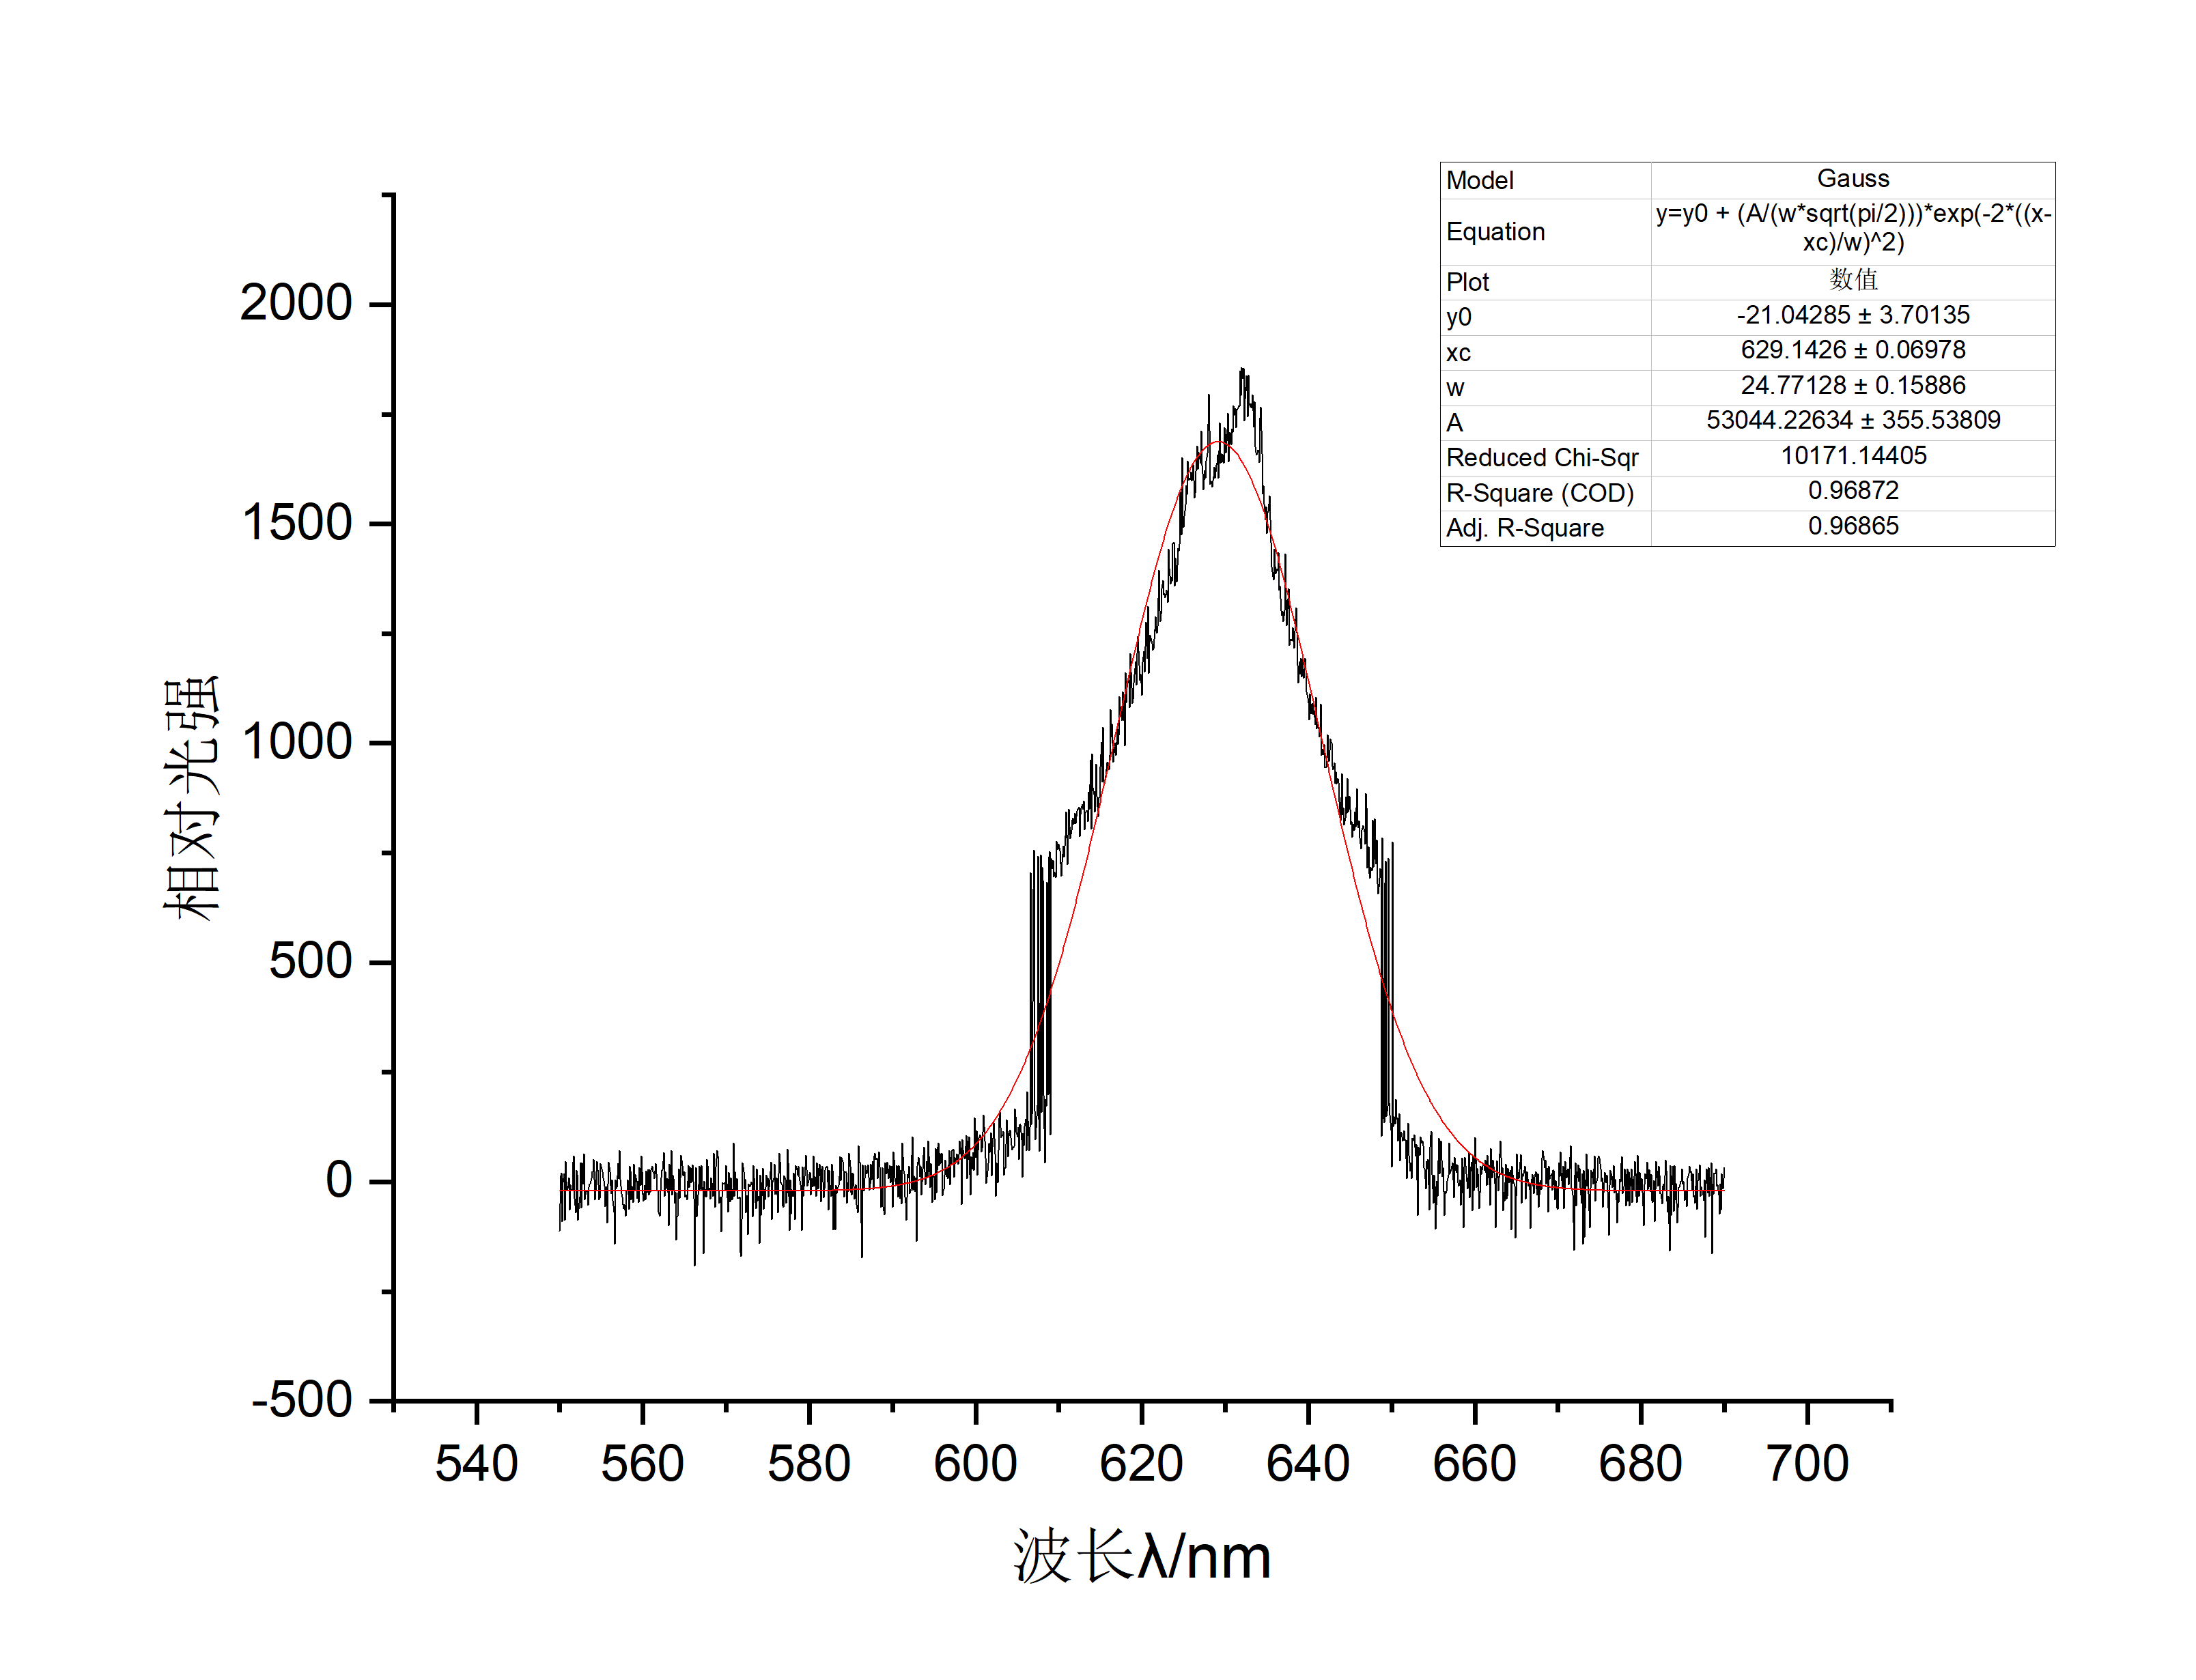
\includegraphics[width=0.33\textwidth]{img//Red.png}
	}
	\subfloat[蓝光]{\label{fig:8.2}
	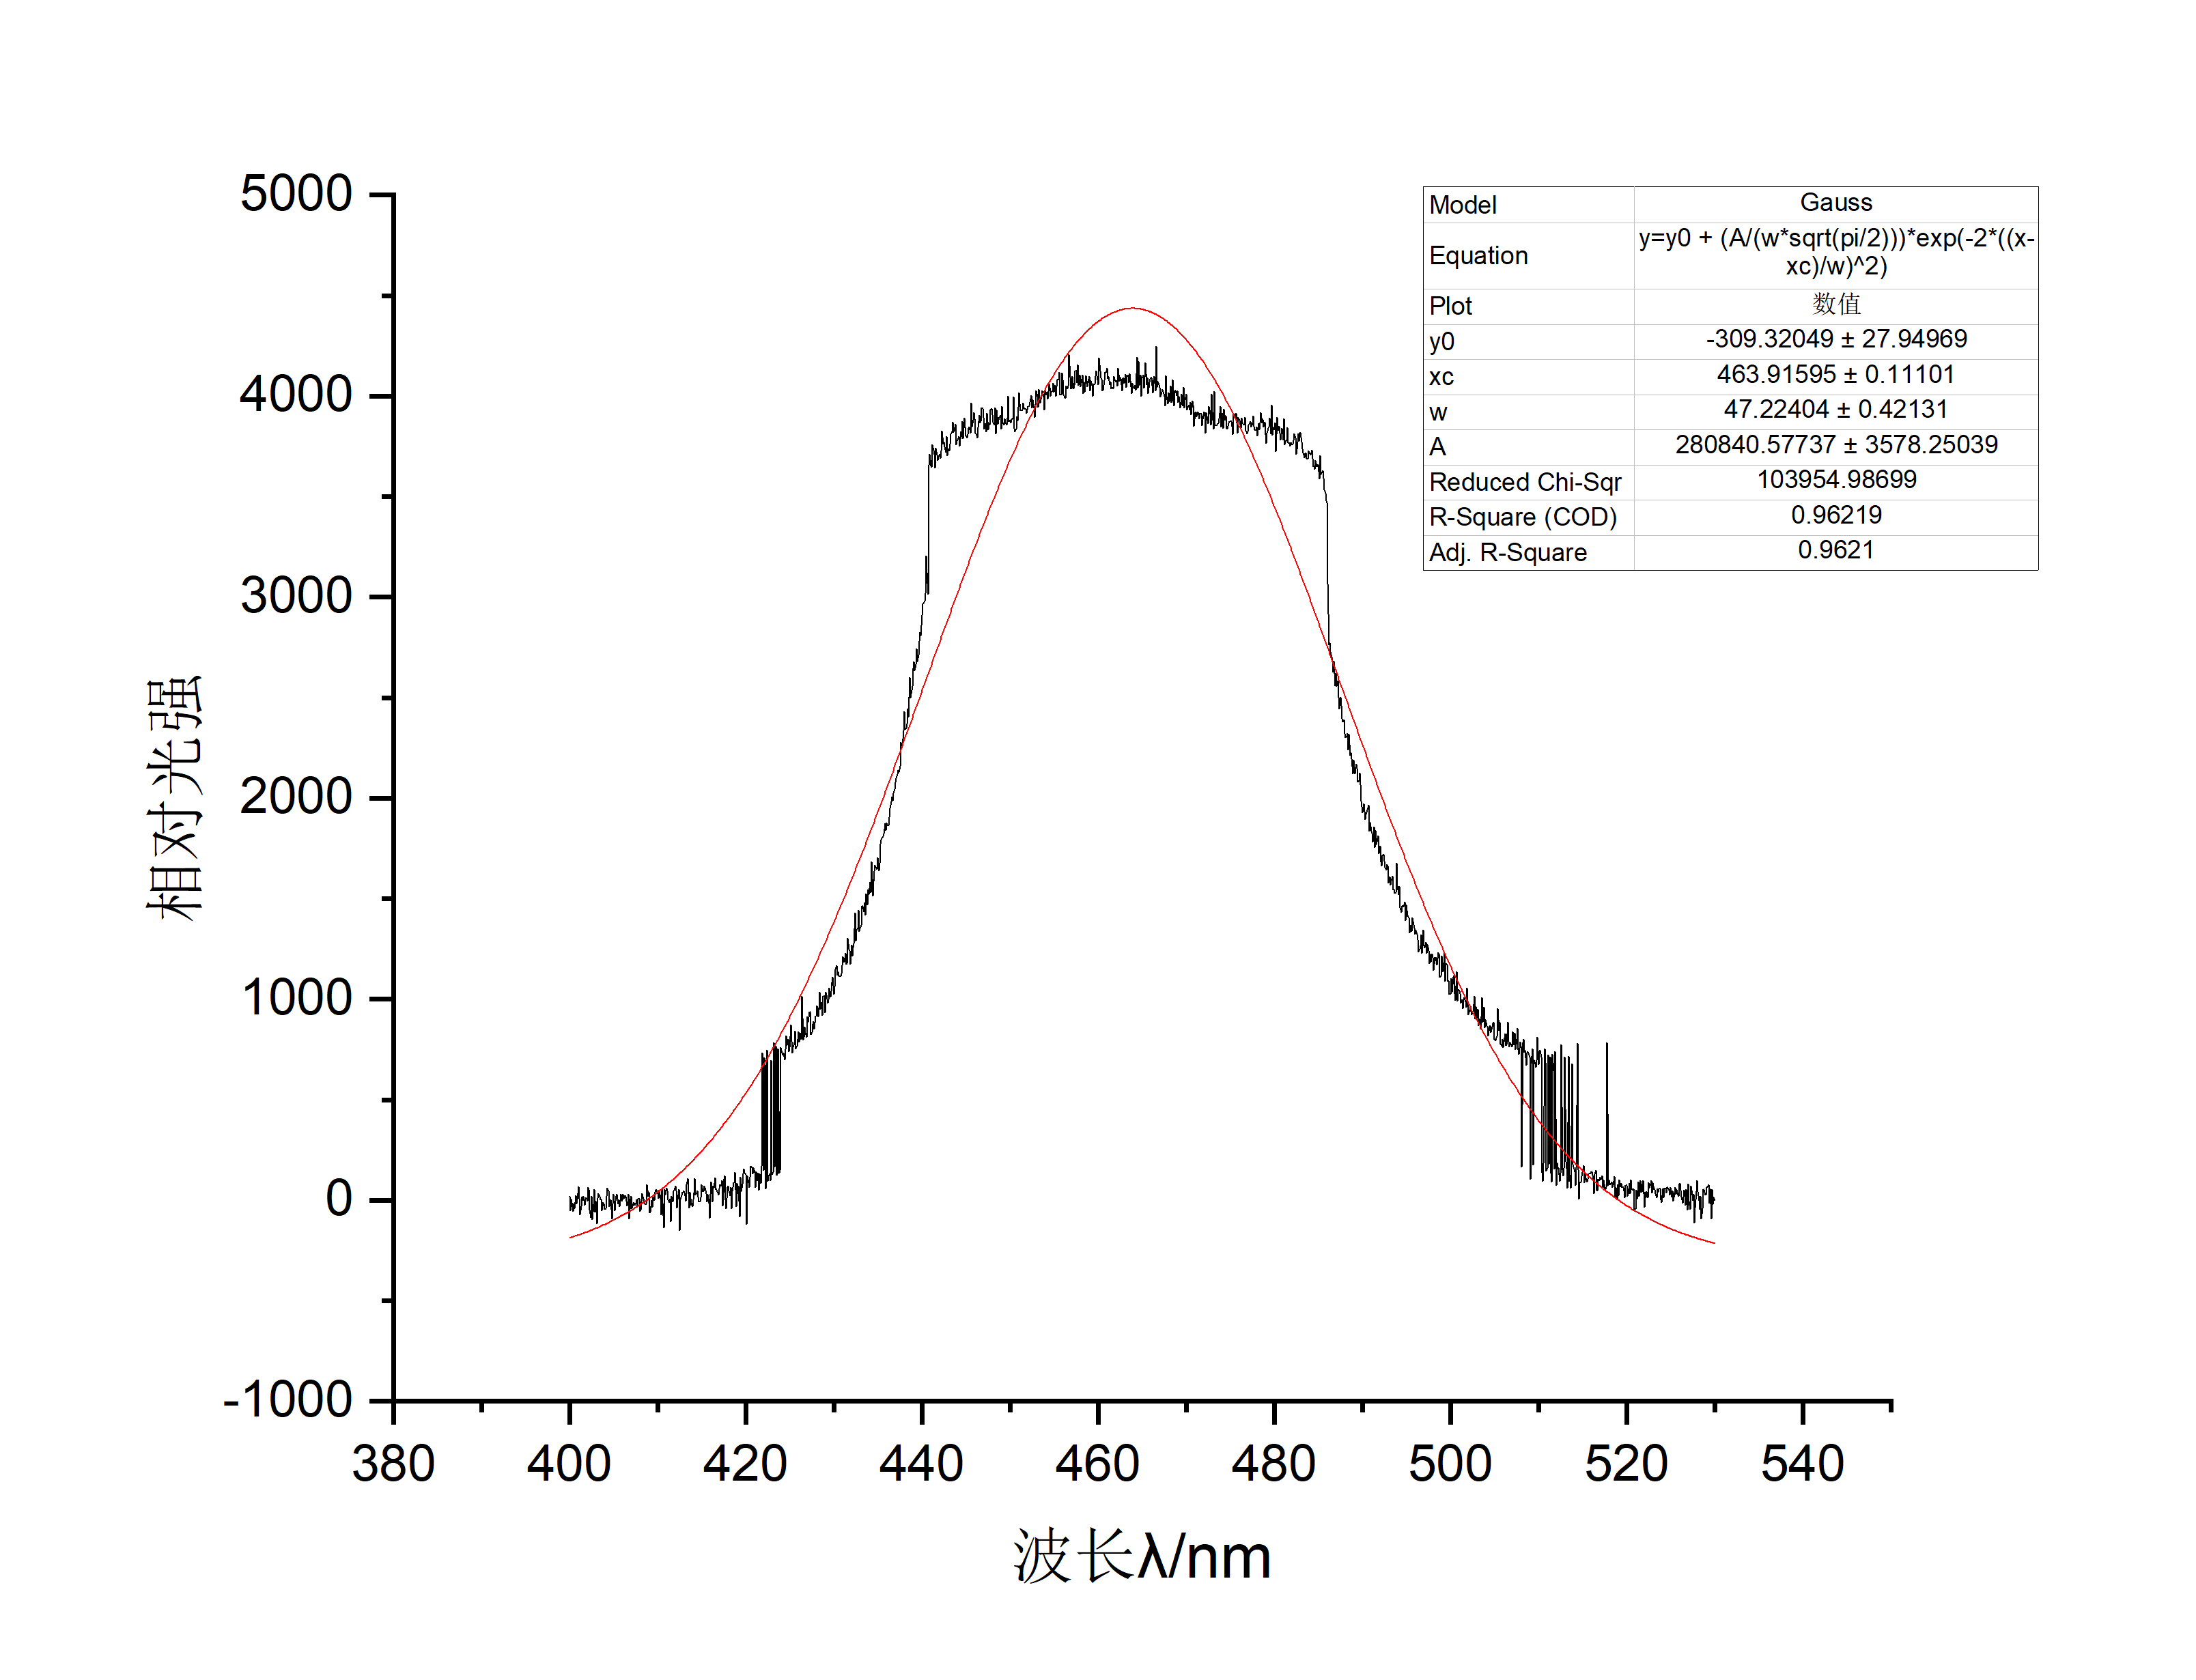
\includegraphics[width=0.33\textwidth]{img//Blue.png}
	}
	\subfloat[绿光]{\label{fig:8.3}
	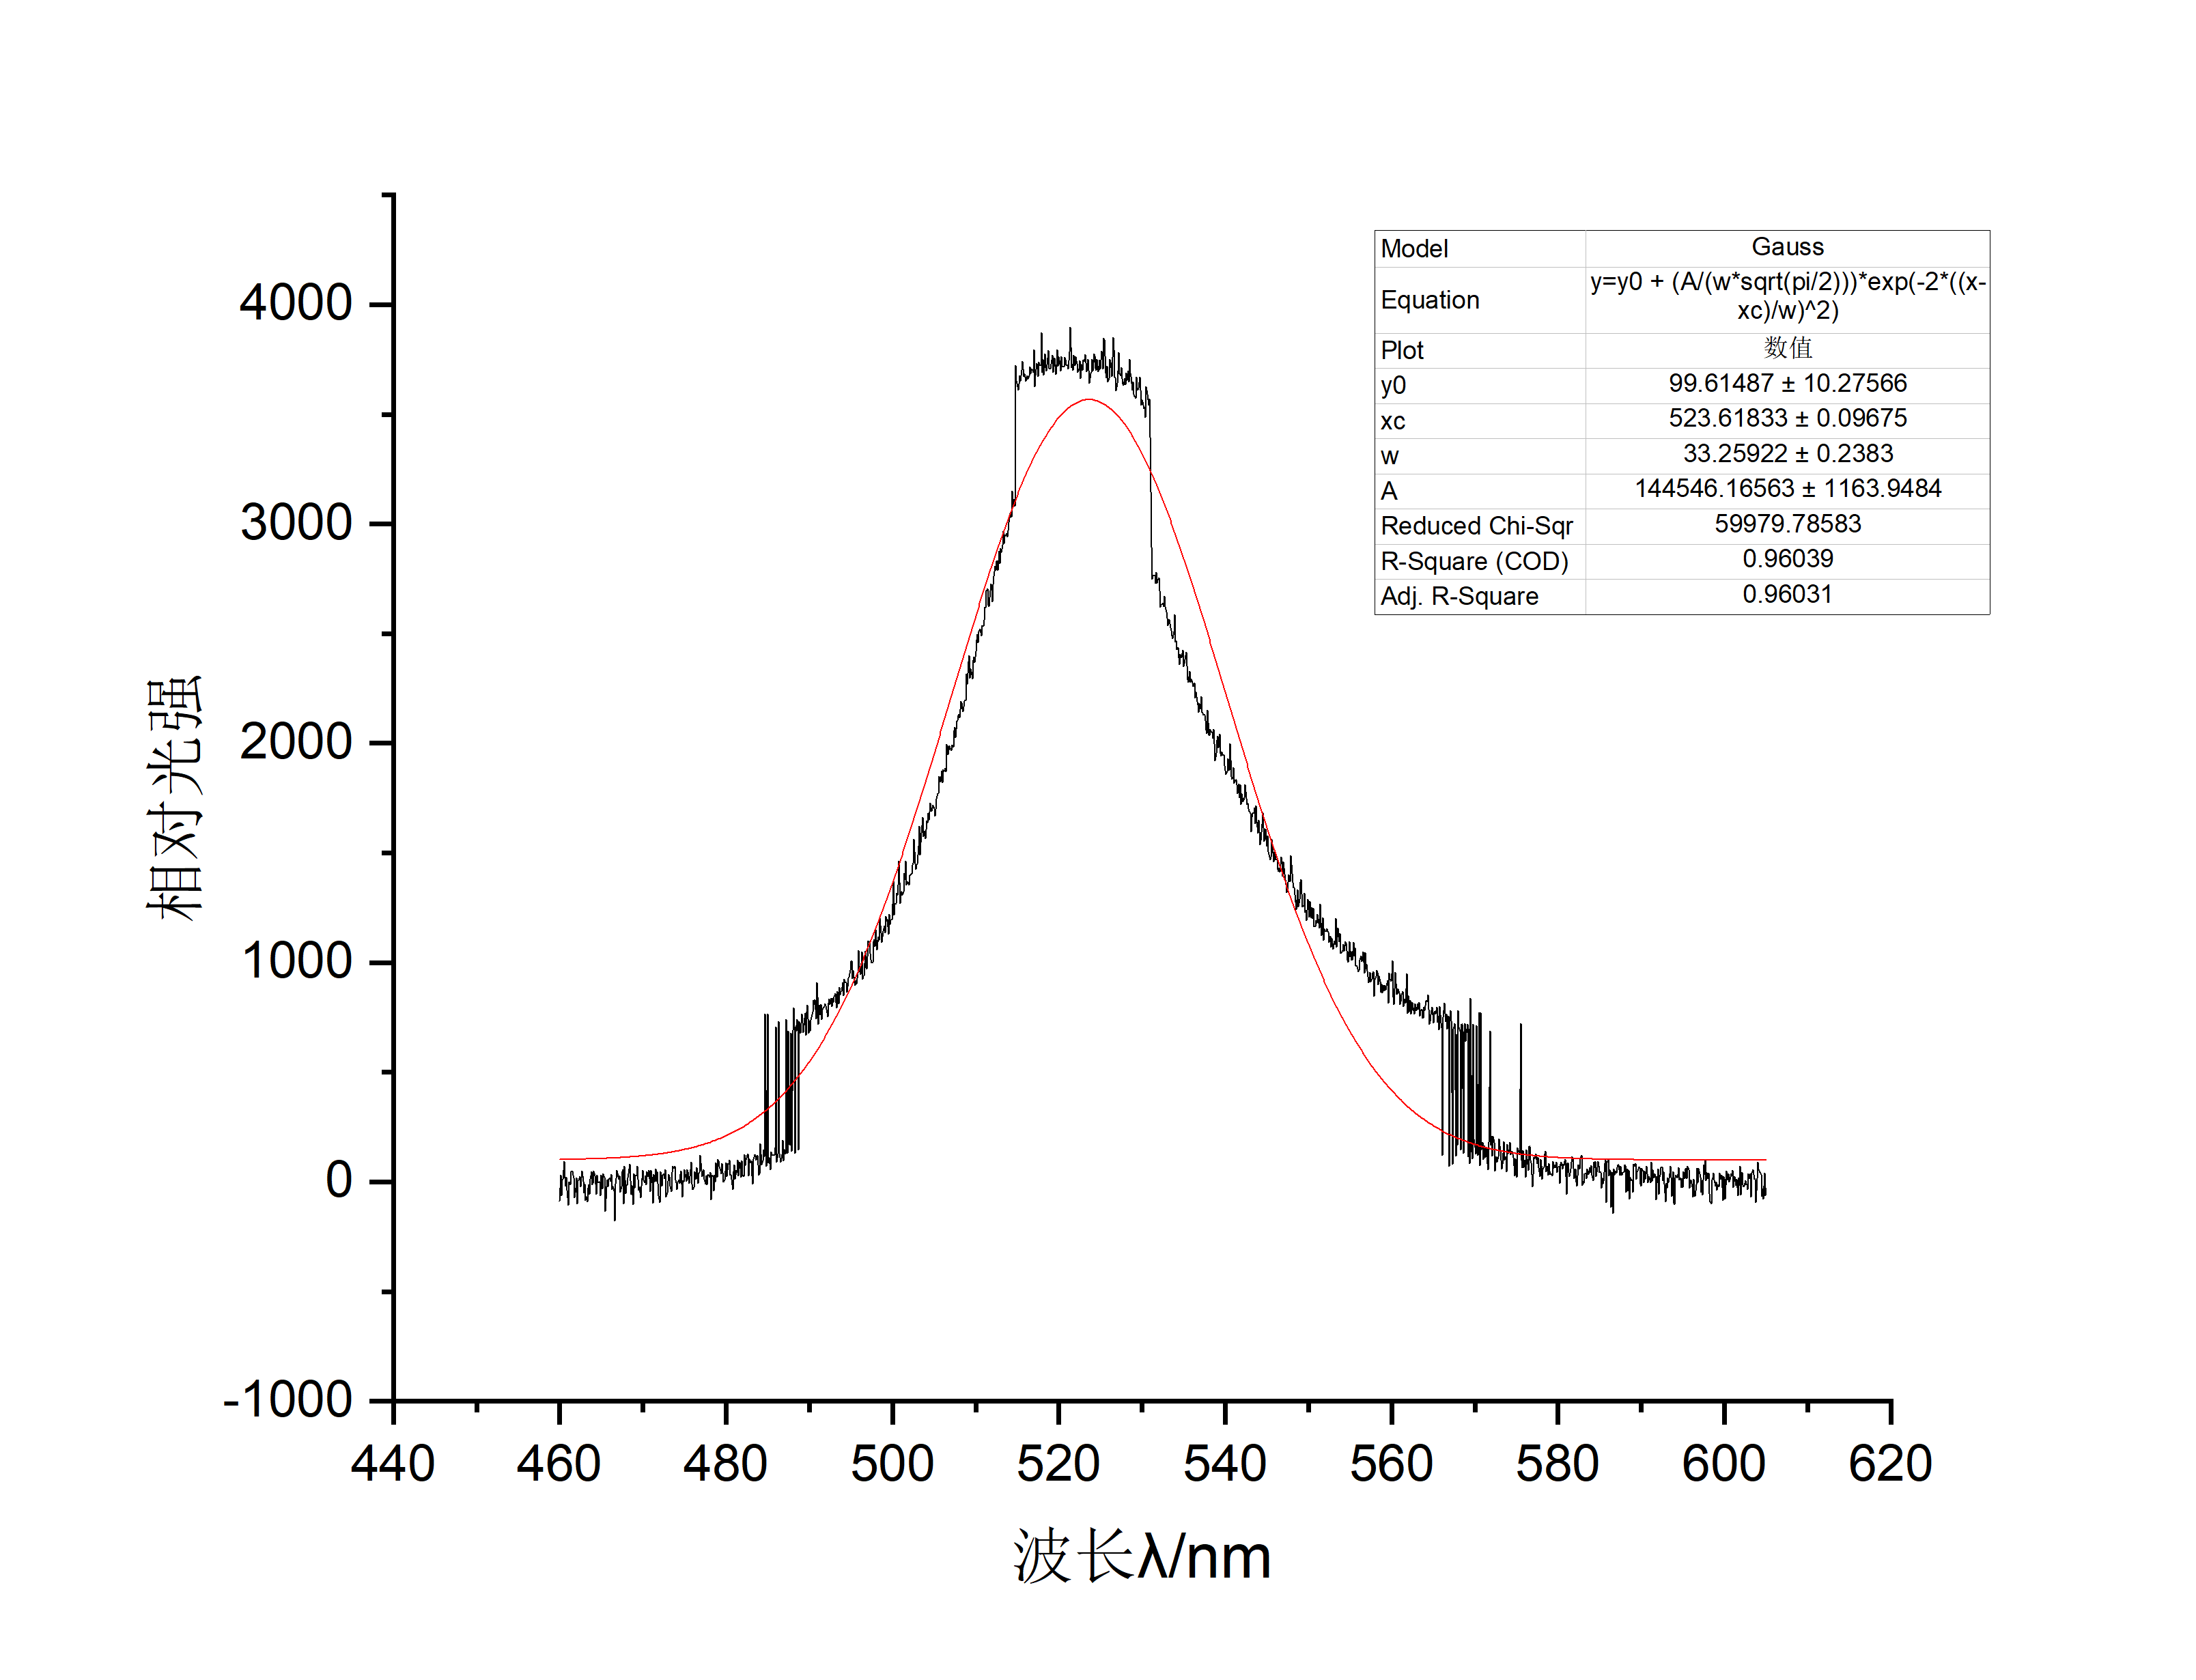
\includegraphics[width=0.33\textwidth]{img//Green.png}
	}

	\subfloat[白光]{\label{fig:8.4}
	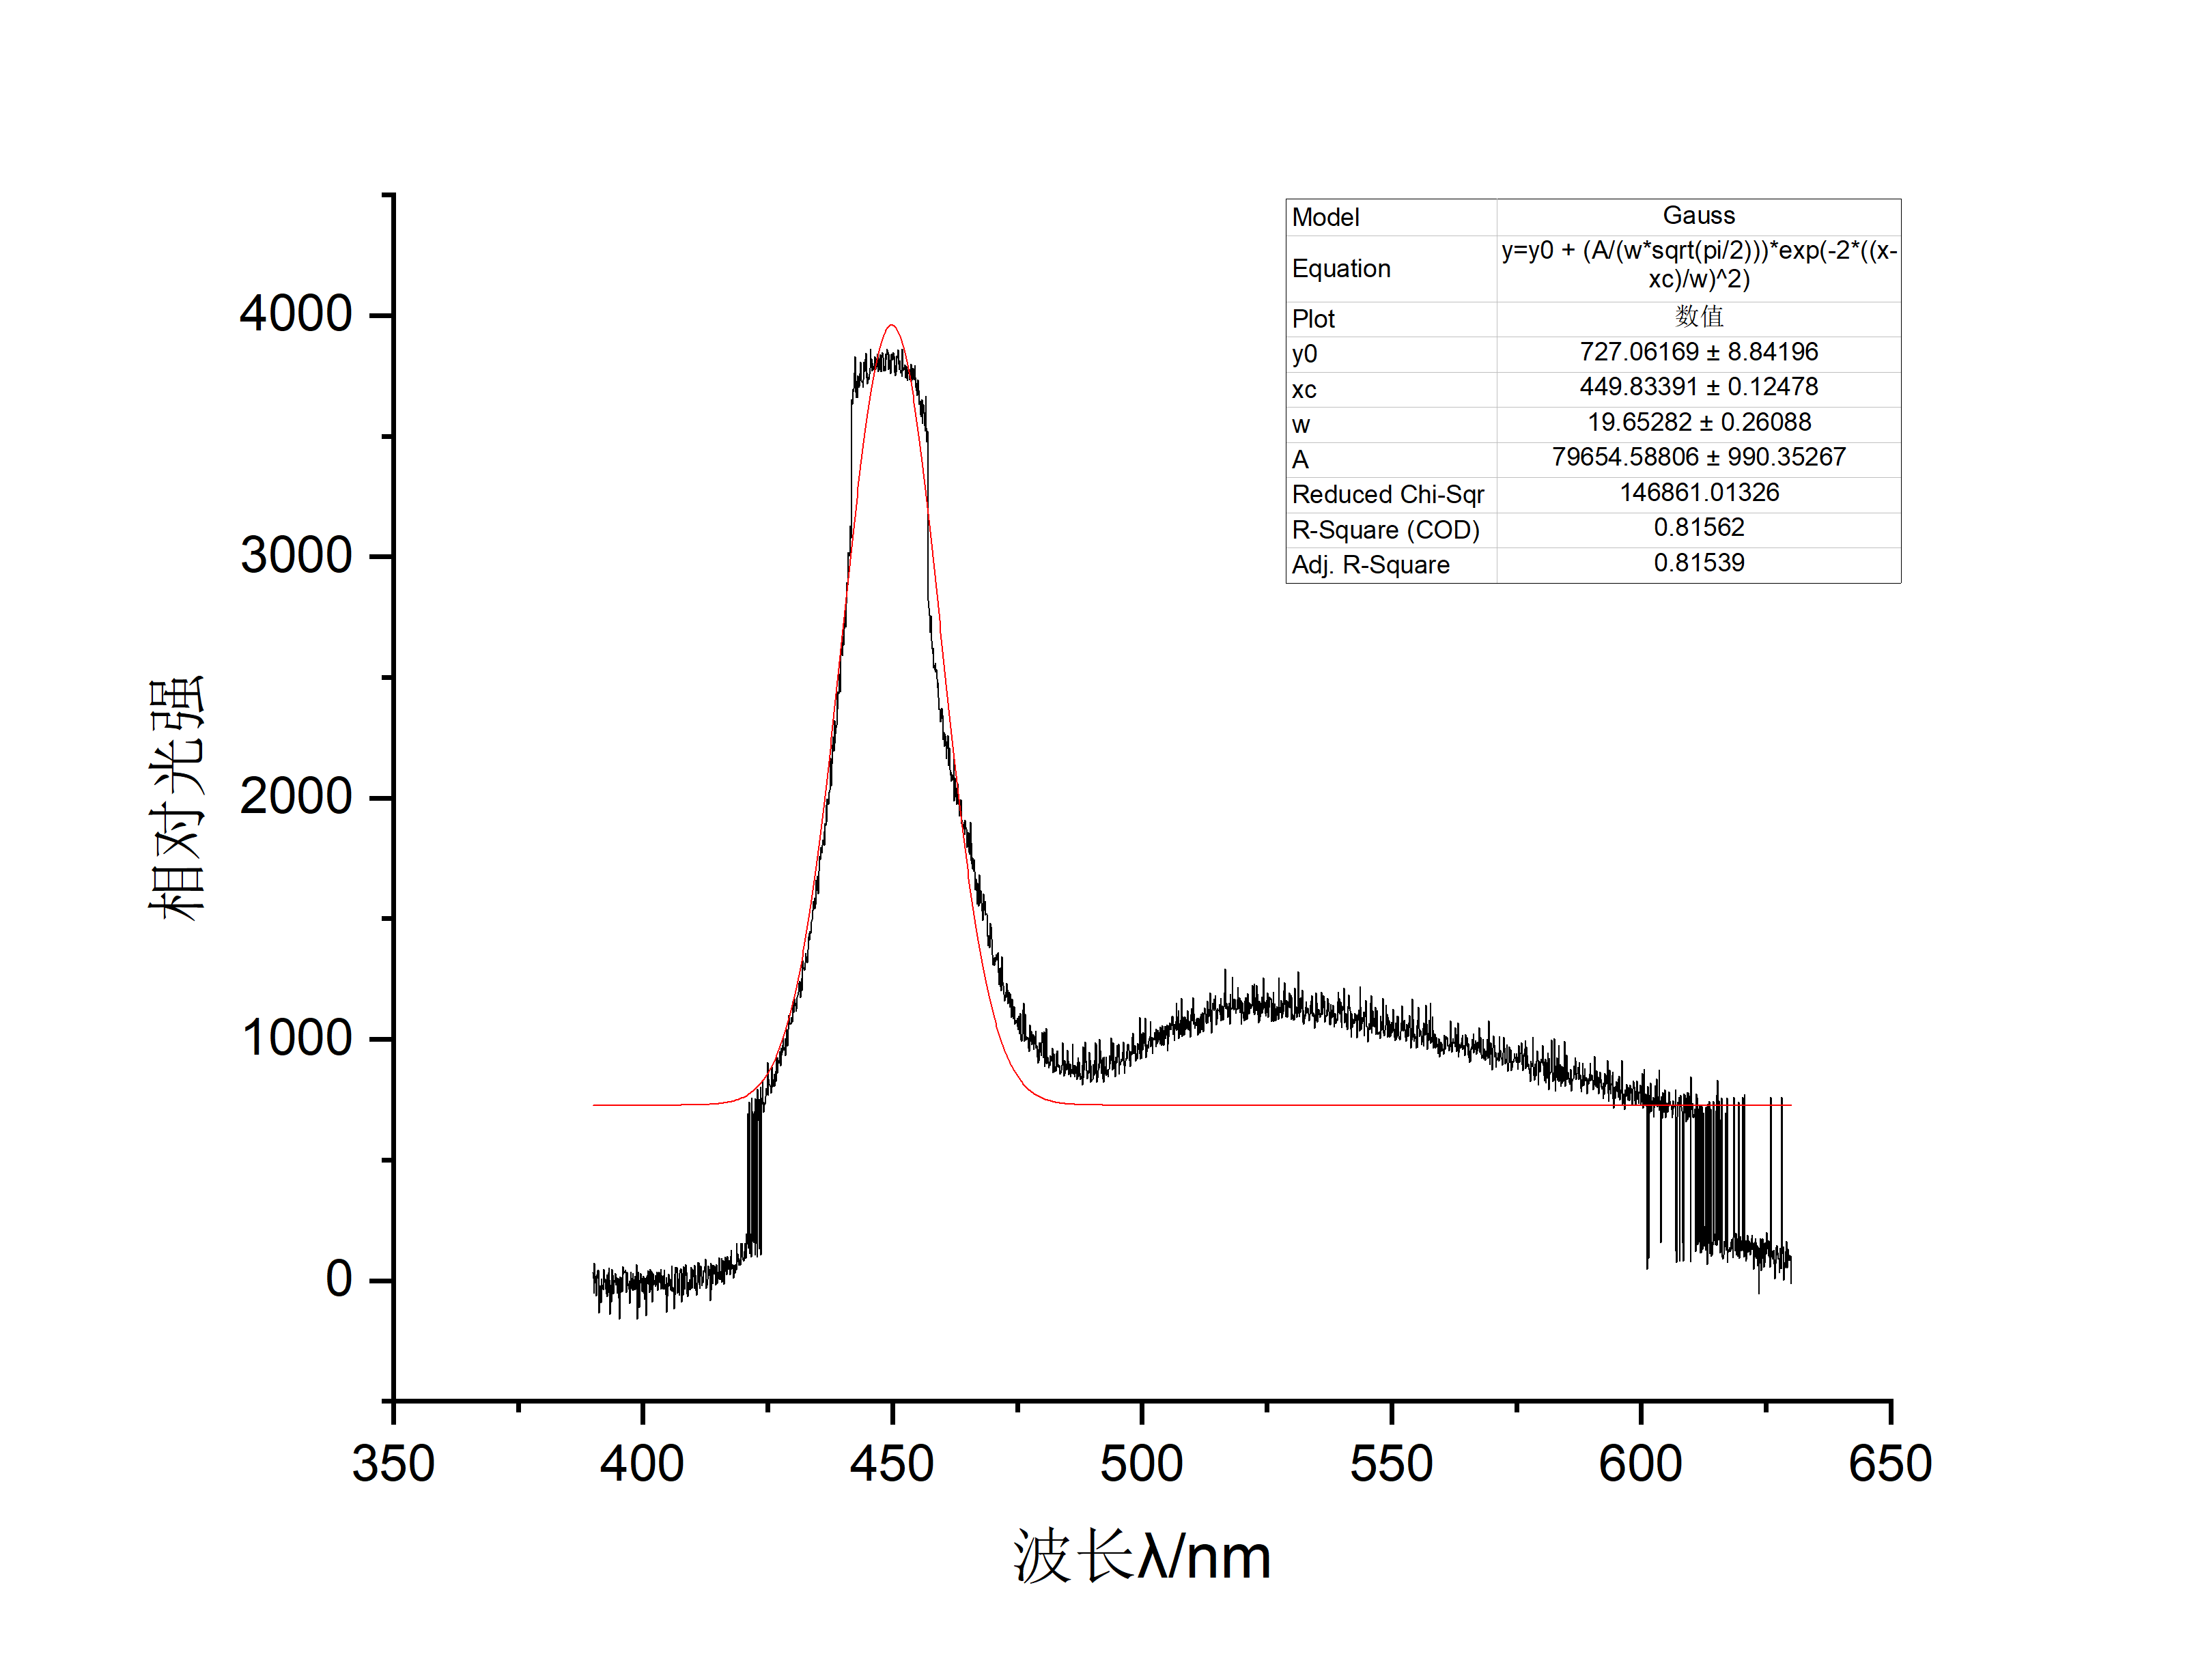
\includegraphics[width=0.33\textwidth]{img//White.png}
	}
	\subfloat[黄光]{\label{fig:8.5}
	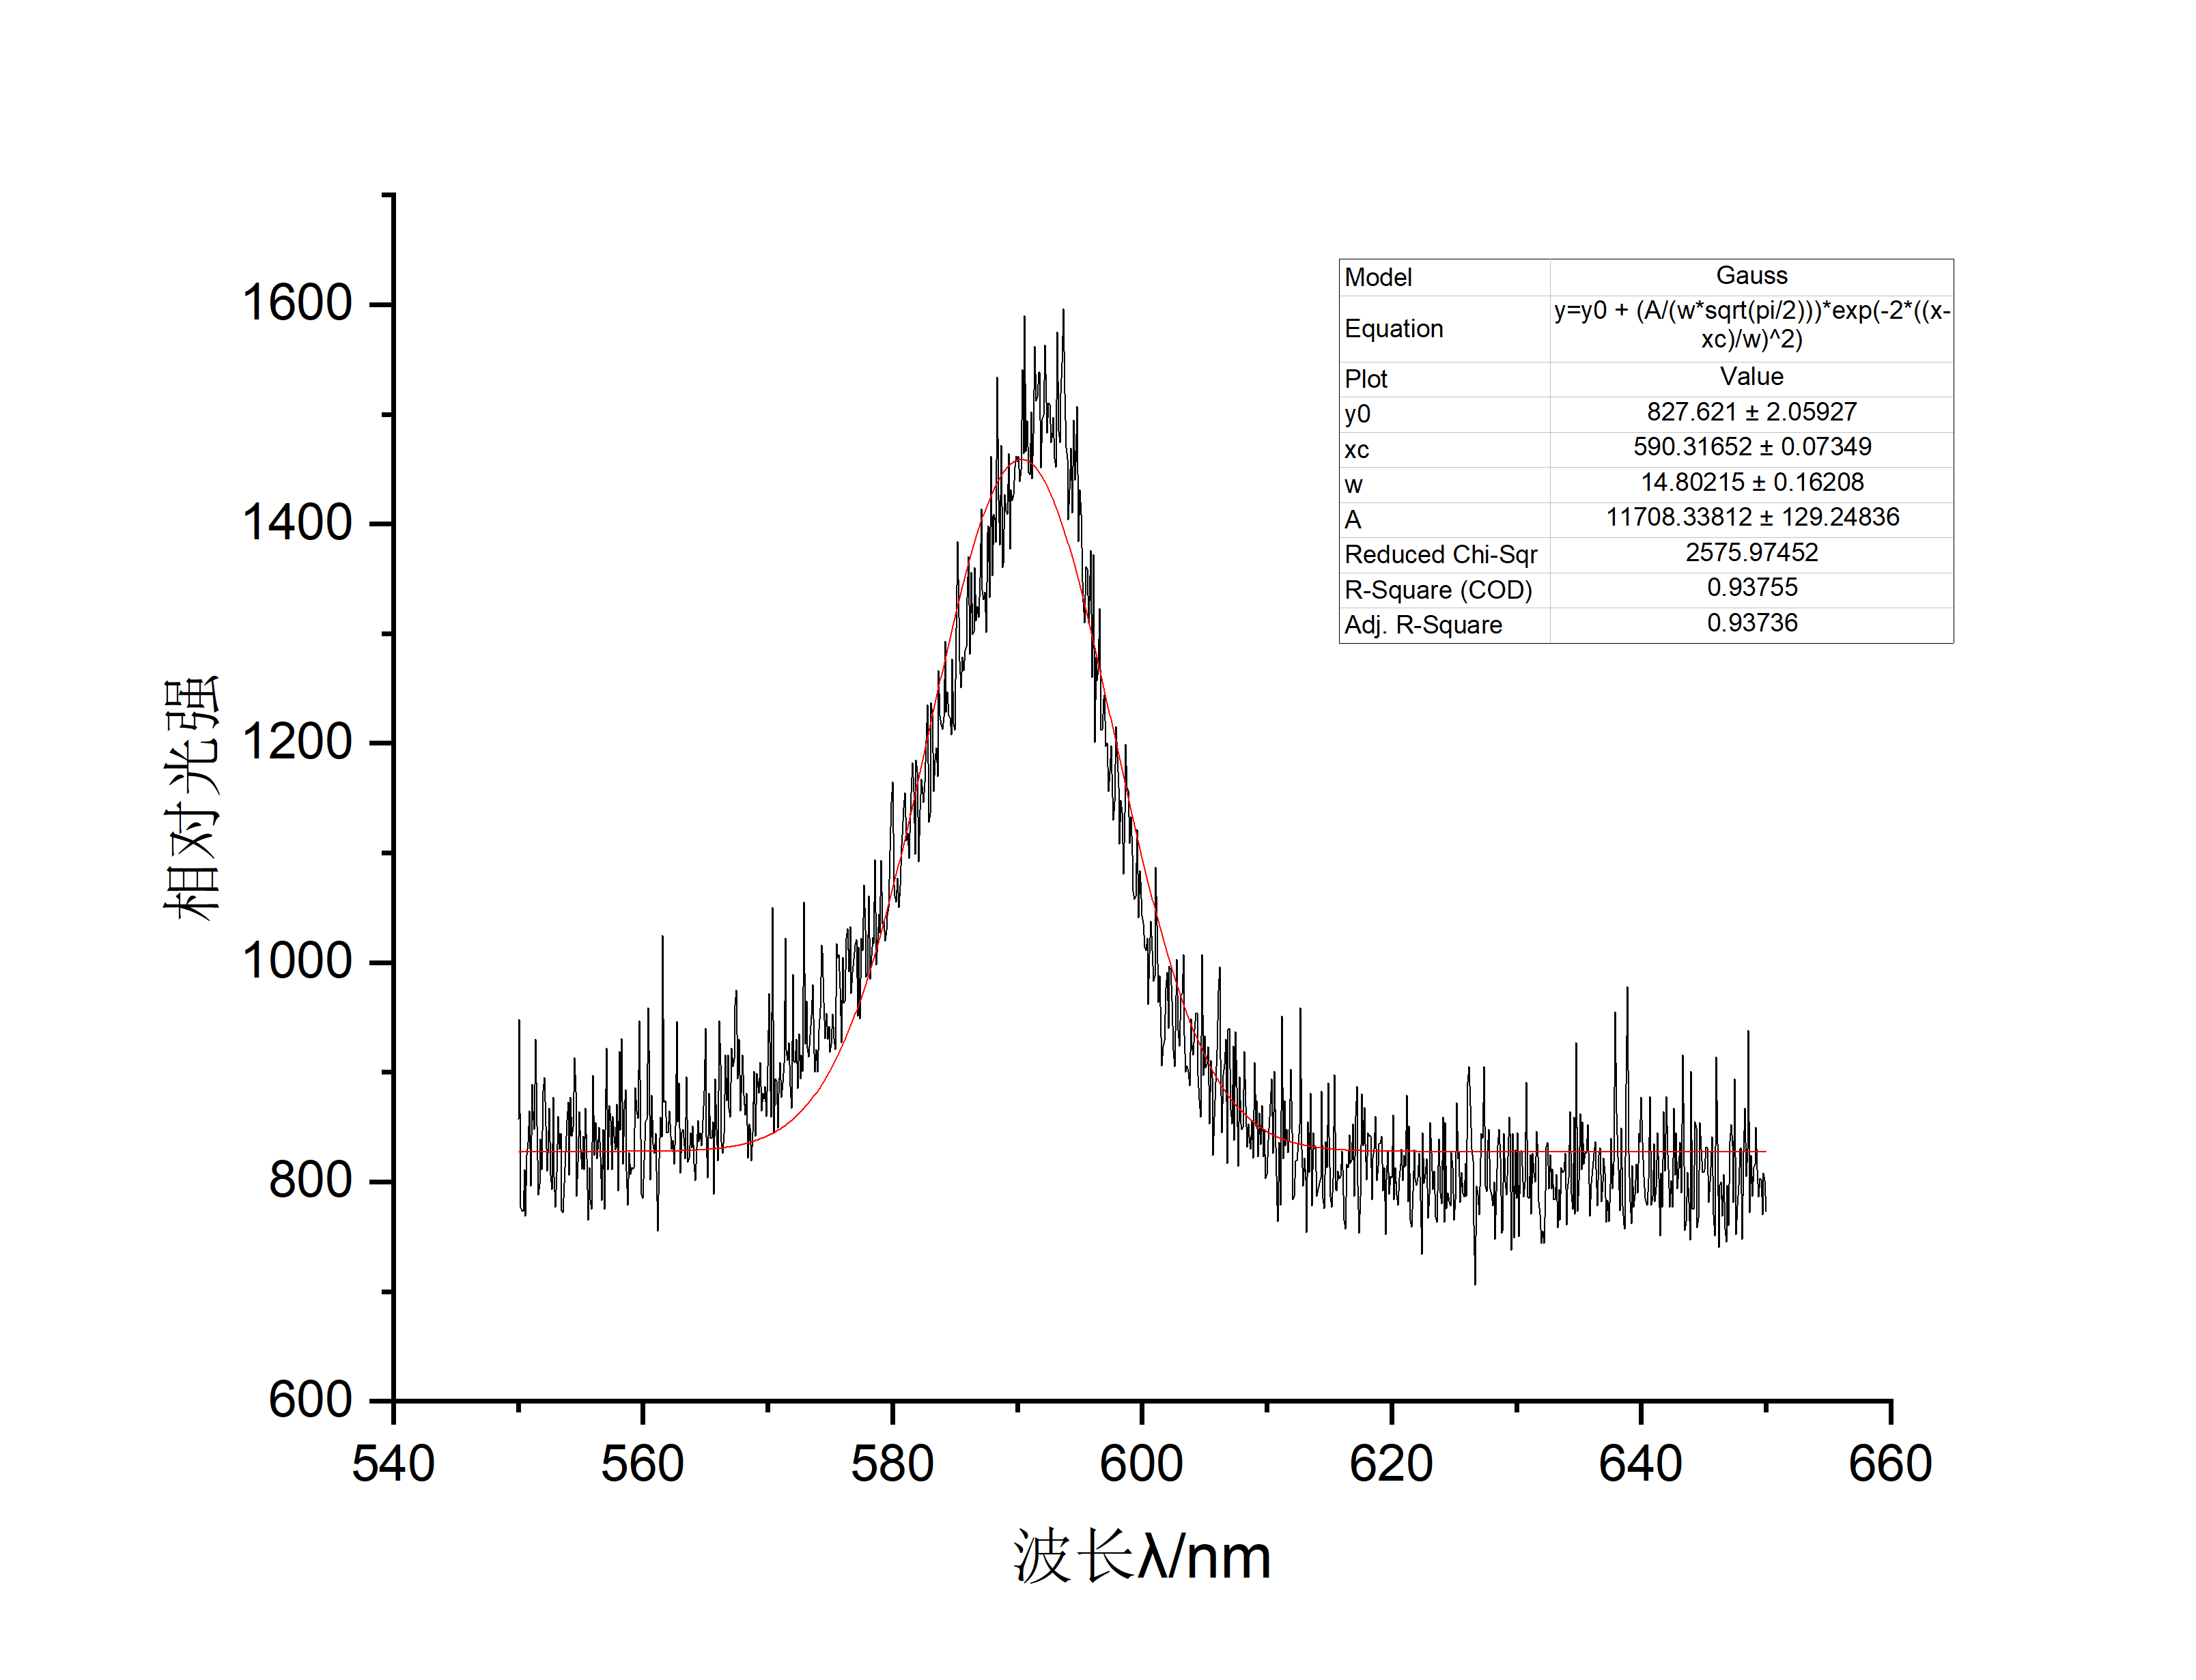
\includegraphics[width=0.33\textwidth]{img//Yellow.png}
	}
	\caption{LED光谱}
	\label{fig:8}
\end{figure}
图中黑色线为测量的吸收光谱,红色线为高斯函数拟合所得曲线。

观察上述光谱可知,除白光外,红、蓝、绿、黄、光谱都只有一个峰。提取峰值得:
\begin{gather*}
	\lambda_{red}=629.14nm\\
	\lambda_{blue}=463.91nm\\
	\lambda_{green}=523.62nm\\
	\lambda_{yellow}=590.32nm\\
\end{gather*}

线性插值法拟合得波长分别位于:
\begin{gather*}
	\lambda^{'}_{red}=0.99519\times\lambda_{red}+2.15853=628.27nm\\
	\lambda^{'}_{blue}=0.99519\times\lambda_{blue}+2.15853=463.84nm\\
	\lambda^{'}_{green}=0.99519\times\lambda_{green}+2.15853=523.26nm\\
	\lambda^{'}_{yellow}=0.99519\times\lambda_{yellow}+2.15853=589.64nm\\
\end{gather*}

而白光光谱波长的两个峰分别位于450nm和520nm处,与蓝光、绿光波长相接近,这是由于白光发光机制决定的。
其发光机制一般为将蓝光LED或紫外光LED所产生的蓝光和紫外光分别转换为双波长或三波长白光,此技术称为荧光转换白光技术。


\subsubsection*{【误差分析】}
\begin{enumerate}
	\item 扫描步长大,没法准确捕捉峰值位置。
	\item Origin软件采集峰值功能不够准确。
	\item 光源本身强度不稳定,导致实验结果出现偏差
	\item 外界光源对实验有影响。
	\item 出入缝宽调节不合适。
\end{enumerate}






\newpage
\subsection*{【思考题】}
\subsubsection*{1. 钠原子光谱有哪些特征?从光谱图上如何判断各谱线所属线系?}
答:钠原子光谱特征:

(1)钠原子光谱分为如下四个线系:主线系、锐线系、漫线系、基线系;

(2)在同一线系内,越向短波方向,相邻谱线波数差越小,最后趋于一个极限;(3)在同一线系内,越向短波方向,谱线强度越小;(4)主线系和锐线系是双线的,漫线
系和基线系是复双重线的。

光谱上判别各谱线线系的方法:

(1)主线系只有钠双黄线在可见光区,其他都在紫外;锐线系和漫线系谱线除第一条在红外区外其他都在可见光区,基线系在红外区

(2)主线系和锐线系是双线的,漫线系和基线系是复双重线的;锐线系各双线波数差都相等;

(3)从谱线的外表上看,主线系强度较大,锐线系轮廓清晰,漫线系显得有点弥漫。


\subsection*{【附录】}
\begin{figure}[htbp]
	\centering
	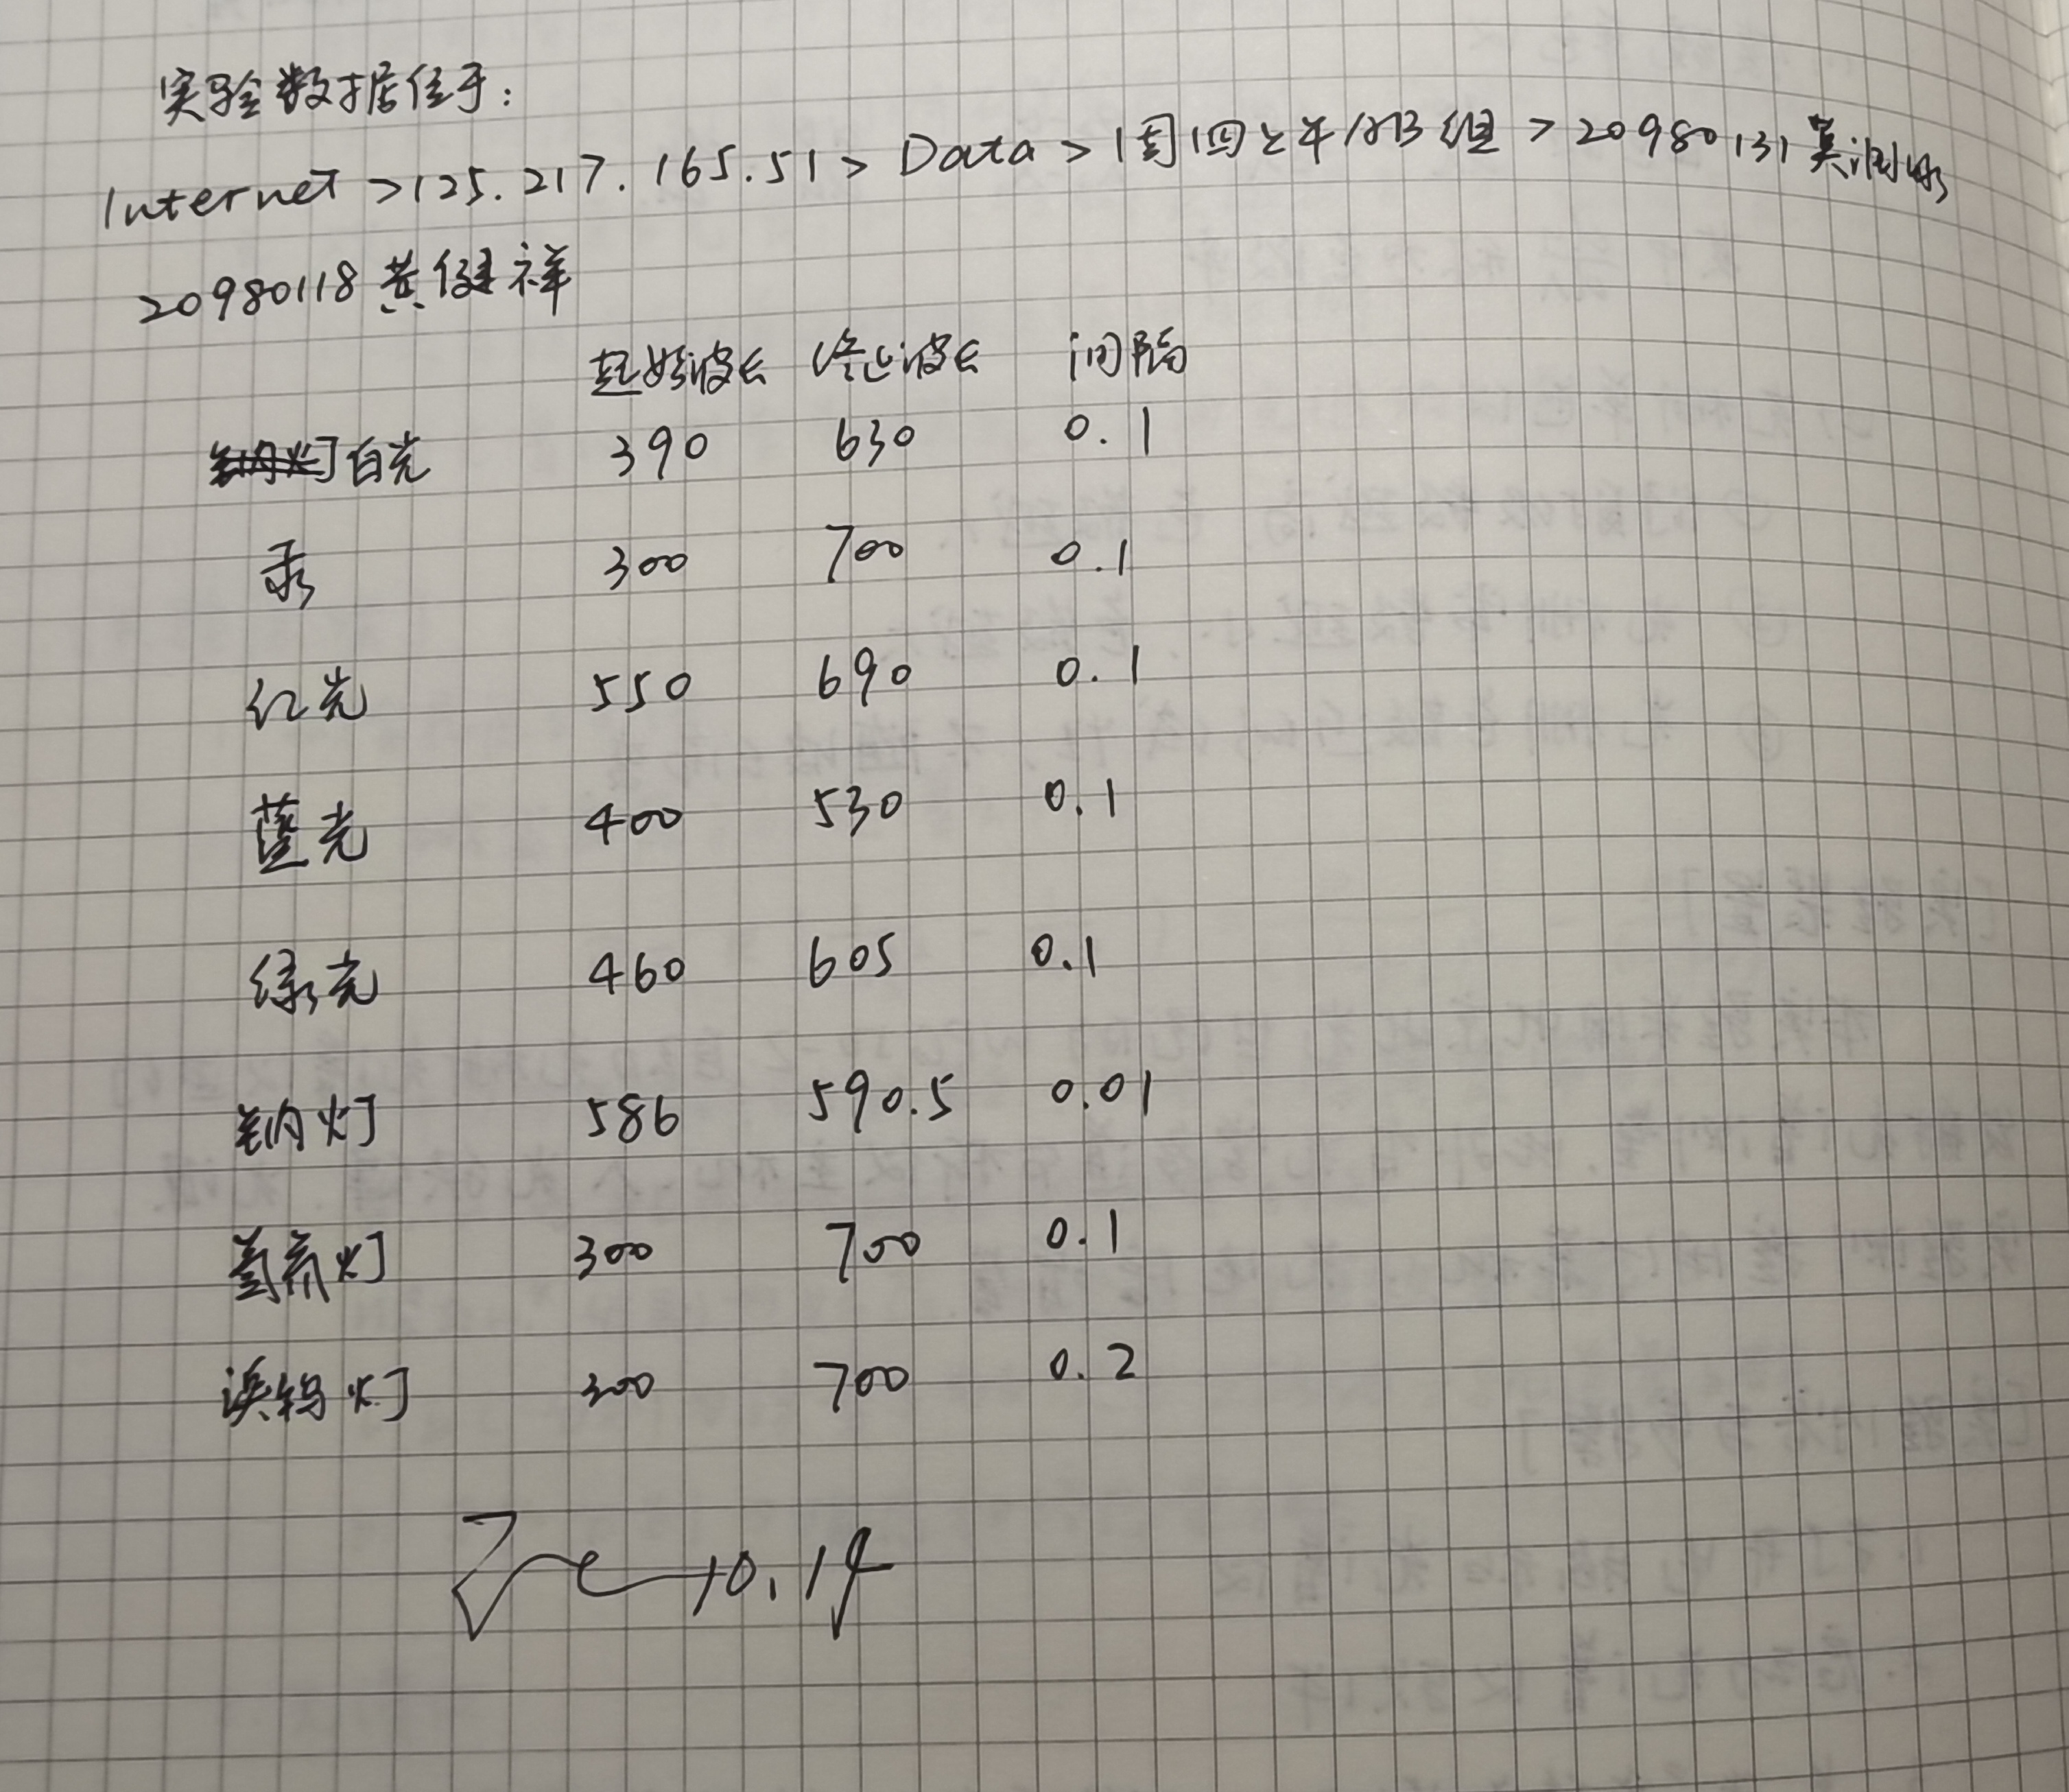
\includegraphics[width=0.6\textwidth]{img//9.jpg}
	\label{fig:9}
\end{figure}
\end{document}
